\documentclass{./packages/homework}
\usepackage{./packages/caratula}
\usepackage{amssymb}

\graphicspath{./files/src/media/}
\renewcommand{\contentsname}{contenidos}
\renewcommand{\refname}{Referencias}
\renewcommand\qedsymbol{$\blacksquare$}
\renewcommand{\lstlistingname}{Algoritmo}% Listing -> Algorithm
\renewcommand{\figurename}{Figura}% Listing -> Algorithm

\lstdefinelanguage{pseudo}{
  morekeywords={
    pre,
    post,
    if,
    while,
    for,
    in,
    out,
    proc,
    inout
  },
  sensitive=false, % keywords are not case-sensitive
  morecomment=[l]{//}, % l is for line comment
  morecomment=[s]{/*}{*/}, % s is for start and end delimiter
  keywordstyle=\color{black}\textbf,
  commentstyle=\color{gray},
  morestring=[b]" % defines that strings are enclosed in double quotes
}

\newcommand{\TODO}[1]{
  {\noindent \color{red} [#1]}
}


\begin{document} 

% caratula
\titulo{TP 2: Análisis de Redes Sociales}
\subtitulo{}
\fecha{Octubre 27, 2022}
\materia{Métodos Numéricos}
\grupo{Grupo 18}

\integrante{Vekselman, Nat\'an}{338/21}{natanvek11@gmail.com}
\integrante{Arienti, Federico}{316/21}{fa.arienti@gmail.com}
\integrante{Manuel Lakowsky}{}{}
\integrante{Brian Kovo}{}{}

\maketitle


% palabras clave y resumen
\addtocontents{toc}{\protect\setcounter{tocdepth}{0}}
\section*{resumen}
\addtocontents{toc}{\protect\setcounter{tocdepth}{3}}
La descomposición de matrices en autovectores y autovalores aparece en una variedad de aplicaciones donde importa caracterizar el comportamiento de un sistema: en el reconocimiento de imágenes, en el análisis de estabilidad de cuerpos rotantes, en el análisis de riesgo de mercado y en el análisis de redes ---por nombrar algunas---. Desde un punto de vista geométrico, se puede considerar a los autovectores como los `ejes' de una transformación lineal, en tanto representan una dirección invariante a la transformación, y a los autovalores como los factores por los que esas direcciones se comprimen, estiran o invierten. 

\vspace{1em}
En este trabajo propondremos una implementación en C++ de un método para el cálculo de autovalores reales, no nulos y en módulo dominantes, y sus respectivos autovectores, en matrices cuadradas. Para algunas matrices particulares, como pueden ser las matrices simétricas definidas positivas, este método nos permitirá obtener todos sus autovalores y autovectores asociados. El mismo se conoce como \textit{el método de la potencia con deflación}. 

A su vez, presentaremos dos aplicaciones concretas de los autovalores y autovectores en el análisis de redes: la medición de centralidad de autovector y corte mínimo en la red del \textit{`Club de Karate'} \cite{Zachary}, y la estimación de una \textit{ego-network} \cite{Leskovec} de Facebook, por medio de la construcción de una matriz de similaridad.  

\vspace{1em}
\noindent Palabras clave: \textit{método de la potencia, deflación de Hotelling, centralidad de autovector, conectividad algebráica, análisis de componentes principales.}

% \newpage
\vspace{2em}

% contenido
\tableofcontents
\newpage

% potencia
\section{Método de la potencia con deflación}
% === INTRO === %

\vspace{1em}
\subsection{Introducción teórica} El método de la potencia con deflación permite aproximar un subconjunto de los autovalores y autovectores asociados a una matriz. Si la misma satisface que todos sus autovalores son no nulos y diferentes en módulo, entonces permite aproximar el conjunto entero. 


\vspace{2em}
\noindent \textsc{Método de la potencia}: el método de la potencia, \textit{Power method} o \textit{Power iteration}, es una técnica iterativa para aproximar el autovector asociado al autovalor en módulo máximo de una matriz cuadrada que satisfaga esta característica ---es decir, tenga un autovalor dominante no nulo---, a partir de la aplicación de sucesivos productos matriciales, descriptos por la siguiente relación de recurrencia:

\begin{equation*}
    b_0\ \text{es un vector aleatorio} : ||b_0|| = 1
\end{equation*}

\begin{equation} \label{potencia}
    b_{k+1} = \frac{\mathbf{A}b_k}{||\mathbf{A}b_k||}
\end{equation}

\vspace{1em}
\noindent donde $|| \cdot ||$ es una norma vectorial.

\vspace{1em}
Se puede demostrar \cite{Burden} que, bajo las condiciones descriptas, si $b_0$ no es ortogonal al autovector asociado al autovalor dominante en módulo de \textbf{A}, $b_k$ convergerá a éste. Lo que es más, se podrá aproximar el autovalor dominante por medio del coeficiente de Rayleigh:

\vspace{1em}
\begin{equation} \label{rayleigh}
    \lambda_{max} = \frac{b_k^t\ \mathbf{A}\ b_k}{b_k^t\ b_k}
\end{equation}


\vspace{3em}
\noindent \textsc{Método de la deflación}: el método de la deflación, por su parte, corresponde a la transformación de la matriz inicial \textbf{A} por una matriz \textbf{B} con autovalores equivalentes, salvo por el autovalor dominante que será anulado. Existen distintos métodos de deflación, entre ellos la deflación de Hotelling y la deflación de Wielandt \cite{Burden}.  

\vspace{1em}
En este trabajo utilizarmos la deflación de Hotelling por su sencillez, a cuestas de un mayor error numérico \cite{Burden}. El mismo consiste en aplicar el método de la potencia para sucesivas matrices que satisfagan la siguiente relación de recurrencia:

\vspace{1em}
\begin{equation*}
    \mathbf{B}_0\ = \mathbf{A}
\end{equation*}

\begin{equation} \label{deflacion}
    \mathbf{B}_{k+1} = \mathbf{B}_{k} - \lambda\ v\ v^t 
\end{equation}

\vspace{1em}
\noindent donde $\lambda$ corresponde al autovalor en módulo máximo estimado por el método de la potencia y $v$ a su autovector asociado.

\vspace{1em}
Se puede demostrar \TODO{citar} que $\mathbf{B}_{k+1}$ contiene los mismos autovalores que $\mathbf{B}_{k}$, salvo el máximo que quedará anulado. %Además, si \textbf{A} es simétrica: 

%\vspace{1em}
%\begin{equation*}
%   \mathbf{B}_k\ \xrightarrow[k\ \to\ n]{}\ \mathbf{0}
%\end{equation*}


%\vspace{1em}
%\noindent donde $n$ es la cantidad de columnas o filas de la matriz. Es decir, el proceso de deflación tenderá hacia la matriz nula.\footnote{Una demostración de esta afirmación se puede encontrar en el apéndice \TODO{XXX}.} 

%$\mathbf{B}_k$ es simétrica\footnote{se puede demostrar que $\lambda v v^t$ es simétrica, por lo que $\mathbf{B}_k$ es simétrica por suma de simétricas.}, en consecuencia diagonalizable y satisface que $\mu_{a}(0) \geq k$. Como la matriz nula es la única matriz diagonalizable con $\mu_{a}(0) = n$, entonces debe ser que $\mathbf{B}_n$ es la matriz nula.  




% === IMPLEMENTACION === %

\vspace{2em}
\subsection{Implementación} Procedemos a detallar una posible implementación para ambos métodos, restringiéndonos al caso de autovalores reales. Definimos:

\begin{align*}
    \text{\textit{deflacion}}&:\ \text{\textit{matriz}}_{n \times n}\ \mathbf{A}\ \times\ \text{\textit{nat} k}\ \times\ \text{\textit{nat} q}\ \times\ \text{\textit{real} t}\
    \longrightarrow\ \text{\textit{vector}}_k\ \times\ \text{\textit{matriz}}_{n \times k}
    \\ \\
    \text{\textit{potencia}}&:\ \text{\textit{matriz}}_{n \times n}\ \mathbf{A}\ \times\ \text{\textit{nat} q}\ \times\ \text{\textit{real} t}\ 
    \longrightarrow\ \text{\textit{real}}\ \times\ \text{\textit{vector}}_n
\end{align*}

\vspace{1em}
\noindent donde $n$ es un natural, \textbf{A} tiene al menos $k$ autovalores reales dominantes en módulo, $0 < k \leq n$, $q$ es un número par\footnote{Esta restricción no es necesaria, pero permite realizar una optimización que se explica en la próxima página.} que representa el máximo de iteraciones a realizar y $0 \leq t$ representa la tolerancia mínima a partir de la que se considera la convergencia de una solución. 

\vspace{1em}
\lstinputlisting[language=pseudo, caption={Pseudocódigo para el método de la deflación.}, label=algo_deflacion]{files/src/.code/deflacion.pseudo}

\vspace{1em}
El algoritmo (\ref{algo_deflacion}.) retornará un vector con los primeros $k$ autovalores en módulo máximos de \textbf{A}, ordenados descendientemente, y una matriz cuyas columnas corresponden, respectivamente, a los autovectores normalizados asociados a estos autovalores. 

\vspace{1em}
Es intersante notar que la $k$-ésima matriz sobre la que se aplicará el método de la potencia ---\textbf{B}$_k$--- tendrá, por definición, un autovalor cero con multiplicidad algebráica mayor o igual a $k$. En el caso en que la matriz inicial sea simétrica, \textbf{B}$_k$ será simétrica\footnote{Por suma de simétricas. Notar que $v v^t$ siempre resulta en una matriz de este tipo.} y, en consecuencia, diagonalizable. Se puede demostrar que la única matriz diagonalizable con multiplicidad algebráica $\mu_{a}(0) = n$ es la matriz nula, por lo que el método de la deflación de Hotelling tenderá hacia ella. Esto nos permite inferir que el error númerico será proporcional a $k$\footnote{En tanto existirá una correlación. Sin embargo, es esperable que otros factores entren en juego: la variabilidad de los autovalores, el número de condición de la matriz, la selección del vector aleatorio inicial, o la cantidad de iteraciones $q$ a realizar, por ejemplo.}. Es decir, los autovalores más chicos de la matriz serán más susceptibles a errores.  


\vspace{2em}
\noindent Por su parte, el algoritmo (\ref{algo_potencia}.) retornará el autovalor de \textbf{A} máximo en módulo y su autovector asociado:

\vspace{1em}
\lstinputlisting[language=pseudo, caption={Pseudocódigo para el método de la potencia.}, label=algo_potencia]{files/src/.code/potencia.pseudo}

\vspace{1em}
Una primera observación importante es que el algoritmo (\ref{algo_potencia}.) no es capaz de distinguir si la selección inicial del vector $v$ es ortogonal al autovector asociado al autovalor en módulo dominante, por lo que una mala selección puede resultar en que el algoritmo falle. Para reducir la probabilidad de ocurrencia, se propone ---heurísticamente--- que se elija cada coordenada del vector de manera pseudo-aleatoria sobre un rango amplio. Por ejemplo, la máxima representación de enteros con signo en 32 bits.

\vspace{1em}
Además, proponemos un modelo diferente al que define la relación de recurrencia de la ecuación (\ref{potencia}.). Su convergencia, en realidad, depende del signo del autovalor en módulo dominante. Si este es negativo, la secuencia será acotada. Se puede demostrar\footnote{\TODO{demostrar}} que la subsecuencia definida por $\{b_k\ :\ k\ \text{es par}\}$ siempre convergerá. 

Lo que es más, esta subsecuencia permite que el método funcione para matrices con distintos autovalores en módulo dominantes, en tanto estos no sean nulos\footnote{\TODO{demostrar}}. El algoritmo (\ref{algo_potencia}.) aprovecha estas observaciones. 

Desde un punto de vista temporal, también permite reducir a la mitad el costo de ejecución (se itera $q / 2$ veces).  




% === EVALUACION === %

\vspace{2em}
\subsection{Evaluación cuantitativa} Procedemos a evaluar nuestra implementación del método de la potencia con deflación en C++ acorde a los algoritmos propuestos.

\vspace{2em}
\noindent \textsc{Error relativo}: medimos el error $\ |\mathbf{A} \mathbf{V} - \mathbf{V} \mathbf{\Lambda}|_1\ $ en función de la cantidad de iteraciones $q$ para 300 instancias de matrices $\mathbf{A} \in \mathbb{R}^{20 \times 20}$ generadas aleatoriamente, donde \textbf{V} y $\mathbf{\Lambda}$ representan ---respectivamente--- las matrices aproximadas de autovectores y autovalores de \textbf{A}, tal que $\ \mathbf{A}\mathbf{V}_i \approx \mathbf{\Lambda}_{ii} \mathbf{V}_i$\ \ \ $\forall i:\ 1\ ...\ n$.  En total, obtuvimos tres millones de mediciones\footnote{El script asociado se puede encontrar en $./experimentos/error\_potencia.py$}.  


\vspace{2em}
\noindent \textsc{Metodología}: se calculó  $\mathbf{\Lambda}, \mathbf{V} = \text{\textit{deflacion}}(\mathbf{A},\ 20,\ q,\ 0)$ y se midió el error relativo para cada una de las matrices sobre cada valor de $q$ en en el intervalo $(0, 1e5)$, de a saltos de $10$.

\vspace{1em}
\noindent Cada caso se generó a través de uno de los siguientes tres procedimientos\footnote{Se utilizó un valor semilla para facilitar la reproductibilidad.}:

\vspace{1em}
\begin{enumerate}
    \item \textit{Matrices Diagonales}: Se generaron cien matrices diagonales \textbf{D} con veinte autovalores en el rango $[-1e5, 0) \cup (0,\ 1e5]$. Los mismos se generaron con el rng \textit{PCG64} de numpy para evitar distribuciones particulares que pudieran influir en la variabilidad de los autovalores.
    \\
    \item \textit{Matrices Diagonalizables}: Se generaron cien matrices diagonalizables $\mathbf{A} = \mathbf{Q}\mathbf{D}\mathbf{Q}^t$ donde cada matriz $\mathbf{D}$ se generó a partir de la metodología (1.) y $\mathbf{Q} = \mathbf{I} - 2uu^t$ se generó a partir de un vector aleatorio $u$ ---con el algoritmo random.rand() de numpy--- tal que $||u||_2 = 1$.
    \\
    \item \textit{Matrices Simétricas Definidas Positivas}: Se generaron cien matrices simétricas definidas positivas de enteros. Para cada caso se generó una matriz aleatoria \textbf{B} con el algoritmo random.randint() de numpy y se procedió a definir la matriz $\mathbf{A} = \mathbf{B} \mathbf{B}^t$. 
\end{enumerate}

\vspace{2em}
\noindent \textsc{Observaciones}: consideramos que la variabilidad de los autovalores y el número de condición de las matrices son variables que afectan de manera significativa al error relativo. El proceso mencionado para la generación de matrices aleatorias fue pensado sobre generadores de números aleatorios para tratar de mantener a ambas variables controladas, en tanto no respondan a ninguna distribución particular que pueda exhibir sus carecterísticas en los resultados del experimento. 


\vspace{2em}
\noindent \textsc{Resultados}. \TODO{experimento}

\newpage

% club de karate
\section{Análisis: Club de Karate}
% === CONTEXTO === %

\vspace{1em}
\subsection{Contexto}

La red del \textit{Club de Karate} es parte de una investigación antropológica \TODO{citar} que estudió las relaciones `políticas' entre los miembros de un club universitario. La misma se realizó durante el desarrollo de un conflicto que terminó por dividir al grupo. La red busca modelar el flujo de información entre sus integrantes por medio de la tripla $(\mathbf{V},\ \mathbf{E},\ \mathbf{C})$, donde $\mathbf{V}$ denota el conjunto de individuos, $\mathbf{E}$ refiere a un grafo no direccionado cuyos ejes representan los vínculos entre los miembros, y $\mathbf{C}$ define la fuerza de estas relaciones ---lo que se podría pensar como ponderaciones sobre los ejes de $\mathbf{E}$---. 

La investigación tuvo como eje central demostrar la capacidad del modelo para predecir la división del grupo por medio del algoritmo de \textit{labeling} de `flujo máximo - corte mínimo' de Ford y Fulkelson \TODO{citar}.

\vspace{1em}
En este análisis utilizaremos sólo la representación matricial de $\mathbf{E}$ para evaluar la importancia de los distintos miembros en la red, y la matriz laplaciana asociada para evaluar el uso de autovectores como predictores de la división del grupo. 




% === CENTRALIDAD DE AV === %

\vspace{2em}
\subsection{Centralidad de Autovector} La centralidad de autovector es una medida que se utiliza en el análisis de redes para medir la `importancia' de los nodos que componen una red, relativa a la importancia de sus conexiones. Dada una matriz de conectividad \textbf{W}, se define:

\vspace{1em}
\begin{equation} \label{conectividad}
    \lambda x = \mathbf{W} x
\end{equation}

\vspace{1em}
\noindent donde $\lambda$ es el autovalor en módulo máximo de \textbf{W}.

\vspace{1em}
Intuitivamente, se puede pensar que la importancia de cada nodo es proporcional a la suma de las importancias de sus vecinos \TODO{citar}. Se puede demostrar \TODO{citar} que, dado las características de esta matriz, el autovector asociado siempre será positivo en coordenadas.

\vspace{1em}
En tanto la red de \textit{Club de Karate}, podemos ver que la aplicación del metodo de la potencia con deflación sobre la matriz de conectividad asociada al grafo $\mathbf{E}$ resulta en el siguiente autovector asociado al autovalor en módulo máximo:

\vspace{1em}
\TODO{presentar vector.}

\vspace{1em}
Vemos que el nodo `1' y el nodo `34' son los más `centrales'. Esto no es casualidad, la red del \textit{Club de Karate} está armada para tener a las dos figuras centrales del conflicto en cada extremo ---el instructor de karate y el presidente del club---, para satisfacer la especificación del algoritmo de `labeling' que utiliza.




% === AV DE LA MATRIZ LAPLACIANA === %

\vspace{2em}
\subsection{Autovectores de la matriz laplaciana} La matriz laplaciana $\mathbf{L} = \mathbf{D} - \mathbf{W}$ ---donde \textbf{D} es una matriz diagonal con elementos $d_{ii} = \sum_j w_{ij}$ y \textbf{W} es una matriz de conectividad--- sirve para medir distintas propiedades en una red. En particular, el mínimo autovalor en módulo no nulo ---llamado de conectividad algebráica, o valor de Fiedler--- permite establecer un criterio sobre el que particionar la red en dos. El autovector asociado a este autovalor designará la pertenencia de un nodo a una u otra partición acorde a su signo. 

\vspace{1em}
Procedemos a analizar qué autovector de la matriz laplaciana asociada a $\mathbf{E}$ permite predecir mejor la división que ocurrió en el \textit{Club de Karate}. Para ello, medimos el valor absoluto de la correlación entre cada autovector y un vector que indica la división que ocurrió en el grupo.

\vspace{1em}
\TODO{presentar solución.}

\newpage

% facebook
\section{Análisis: Red `Ego'}
% === CONTEXTO === %

\vspace{2em}
\subsection{Contexto} 

Una \textit{ego-network} \cite{Leskovec} es una red compuesta por las amistades que existen entre los amigos de un individuo, el `ego'. Estas redes son centrales para aplicaciones como Facebook, Google+ o Twitter. 

En particular, dada una red `ego', resulta de interés poder identificar los circulos sociales ---conjuntos, disjuntos y anidados--- a los que pertenece un usuario. Leskovec \cite{Leskovec} propone un método de aprendizaje no supervisado para lograr inferirlos, que se nutre de la siguiente información: un grafo \textbf{E} (la red) ---donde se espera que exista una correlación fuerte entre un círculo y la densidad de conexiones entre los nodos que lo componen--- y un conjunto de atributos \textbf{C}, para cada nodo ---donde se espera una correlación entre un círculo y la similaridad de los atributos de los nodos que lo componen---.

\vspace{1em}
En este análisis estimaremos \textbf{E}, una red `ego' proveniente de Facebook, por medio de la construcción de una matriz de similaridad que utilice los atributos definidos en \textbf{C}. También, buscaremos reducir su dimensionalidad por medio del análisis de componentes principales.

% === SIMILARIDAD @ ATRIBUTOS === %

\vspace{2em}
\subsection{Matriz de similaridad}

Queremos generar una aproximación de nuestra red `ego' original \textbf{E} en base a los atributos en \textbf{C} de los usuarios que la componen. Es decir, buscamos un método que nos permita comparar los atributos de dos nodos diferentes y, bajo algún criterio propuesto, conectarlos o no en fin de replicar nuestra red verdadera. 

Intuitivamente, una forma de adivinar si dos usuarios se encuentran conectados en una red es contando la cantidad de atributos que comparten. Se podría pensar que si coinciden en muchos existe una mayor probabilidad de que pertenezcan al mismo círculo, mientras que sino podría ser que ni siquiera se conozcan. Las estructuras que utilizaremos para replicar esta línea de pensamiento son las \textit{matrices de similaridad}, las cuales dado un conjunto de datos $X$ aplican una función a cada par de datos $ij$.

\begin{equation}
    S_{ij} = f(X_i, X_j)
\end{equation}

Nuestra tabla de atributos\footnote{La misma puede encontrarse en \textit{./catedra/ego-facebook.feat}.} es tal que la primera columna contiene los tags correspondientes a cada usuario, y el resto de las columnas forman \textbf{C}, donde la $fila_i(\textbf{C})$ son los atributos del usuario $tag_i$. Tomemos entonces nuestra matriz de similaridad $\textbf{S} = \textbf{CC}^{t}$, tal que $\textbf{S}_{ij}$ expresa la similaridad entre la $tag_{i}$ y $tag_{j}$ computando el producto interno de sus respectivos atributos. Con esta información podemos luego proponer diferentes umbrales $u$ entre el menor y mayor valor en \textbf{S}, y establecer que $\textbf{S}_{ij} > u$ indica que los $tag_{i}$ y $tag_{j}$ están conectados en nuestra aproximación. 

Procedemos a mostrar los resultados obtenidos. Tomando $u \in [min{\textbf{S}_{ij}},\ max{\textbf{S}_{ij}}) = [0, 22)$, $u \in \mathbb{Z}$, obtuvimos 22 diferentes aproximaciones de \textbf{E}.
Obsérvese que cuanto más alto sea el umbral, menores conexiones tendremos en nuestro grafo aproximado. En particular, con $u = 0$ se obtiene un grafo donde todos los usuarios están conectados entre sí, y con $u > 12$ grafos con ninguna arista. Nos enfocaremos entonces con los asociados a $u \in [0, 12]$, ya que son los que revelan información de interés.

\vspace{1em}

\begin{figure}[!htbp]
    \centering
    \subfloat[Original]{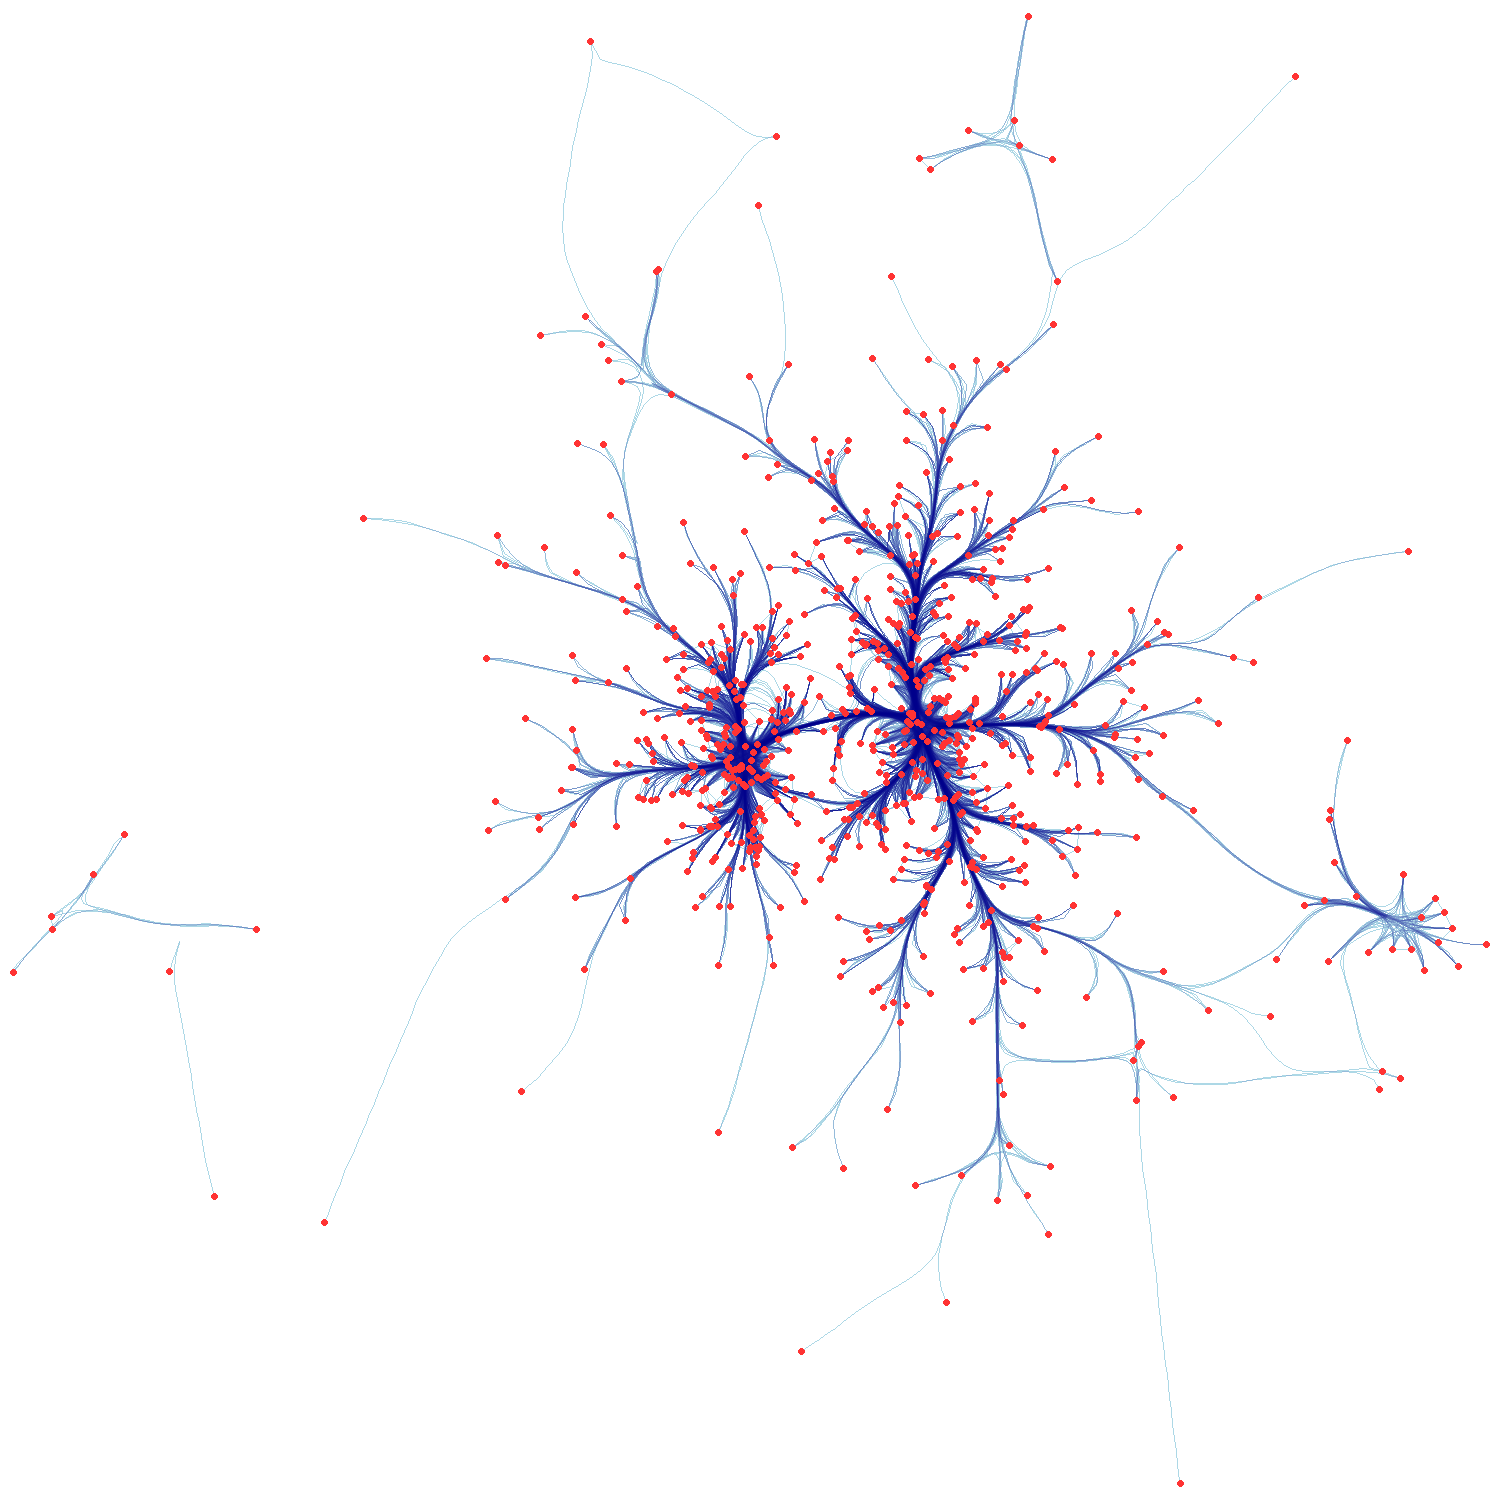
\includegraphics[width=.25\textwidth]{/files/src/.media/ego/grafo_forceatlas2_facebook.png}}\hfill
    \subfloat[$u = 0$]{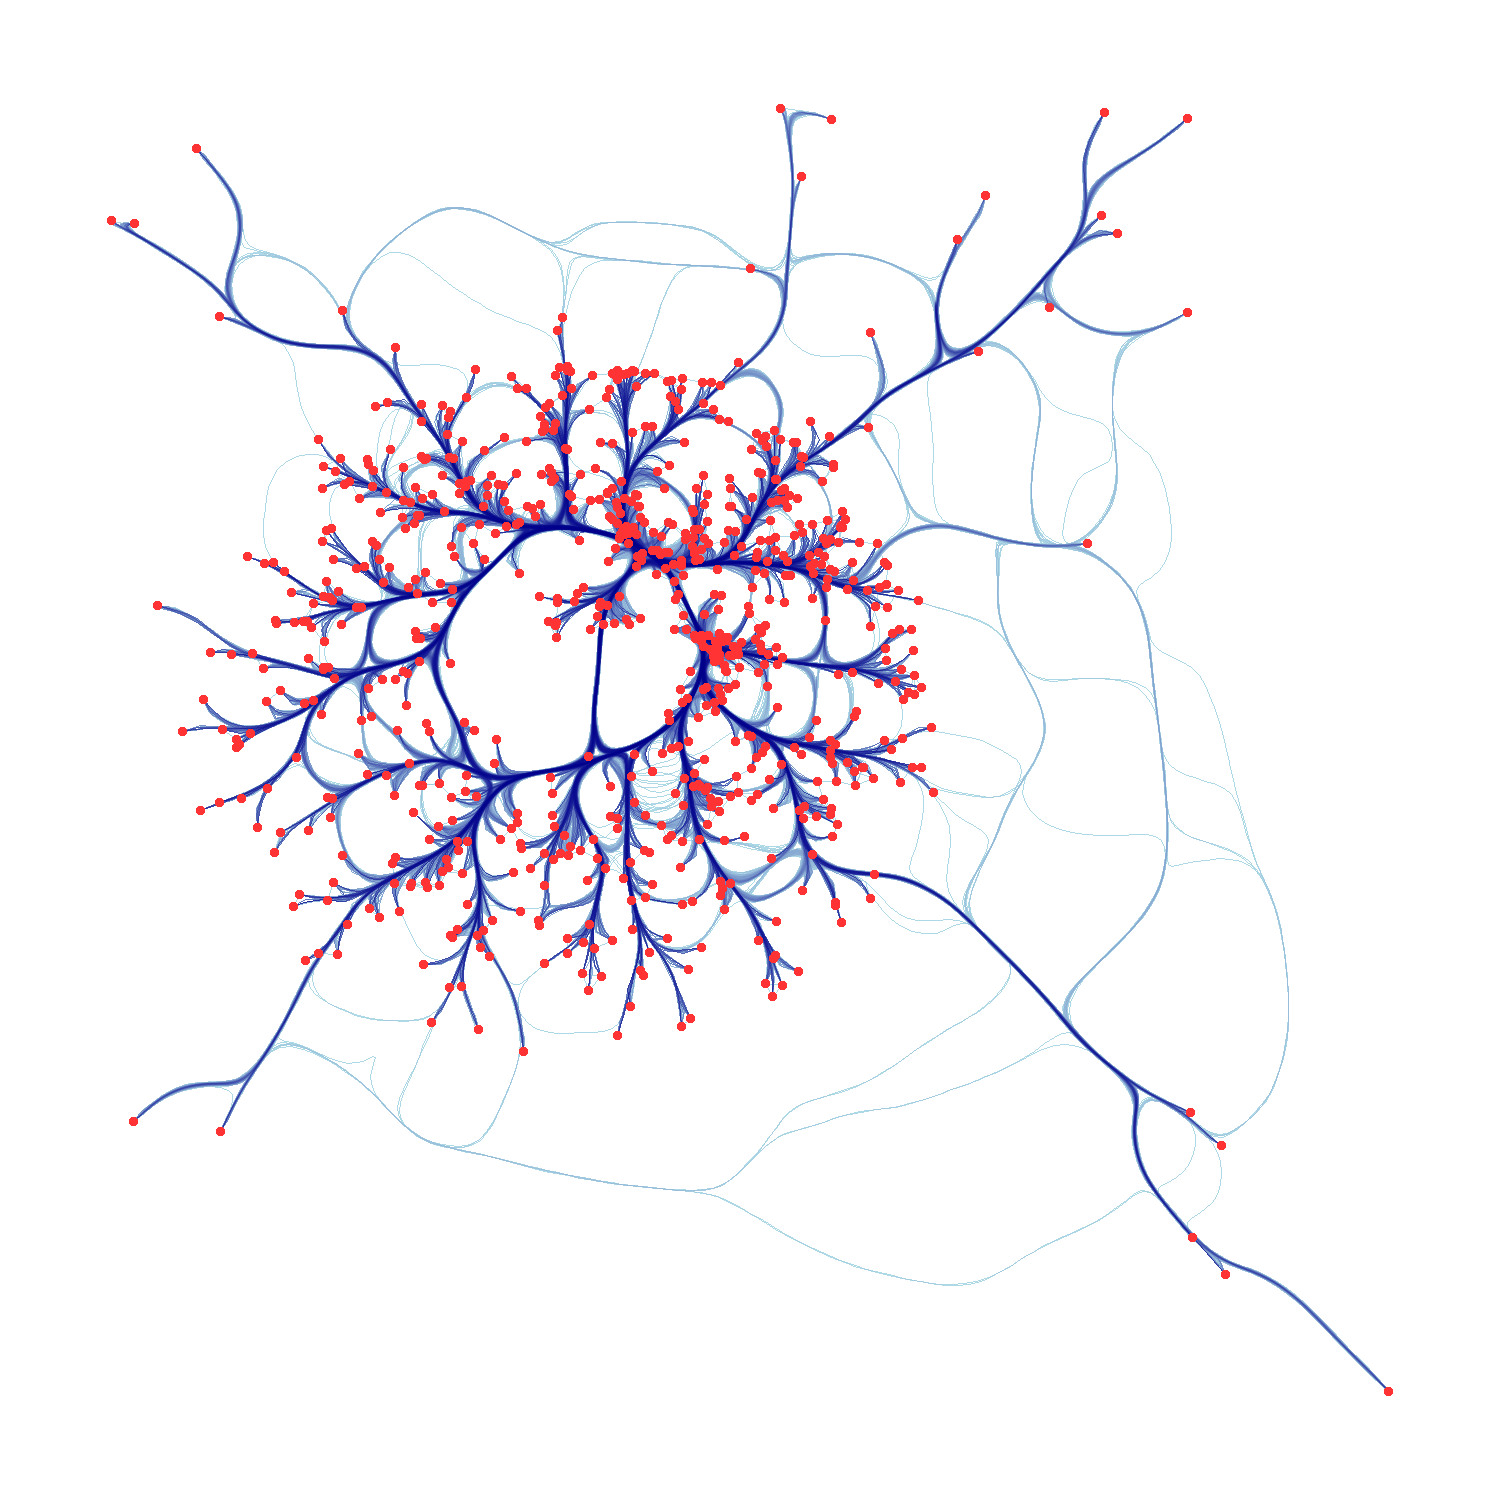
\includegraphics[width=.25\textwidth]{/files/src/.media/ego/grafo_forceatlas2_0.png}}\hfill
    \subfloat[$u = 1$]{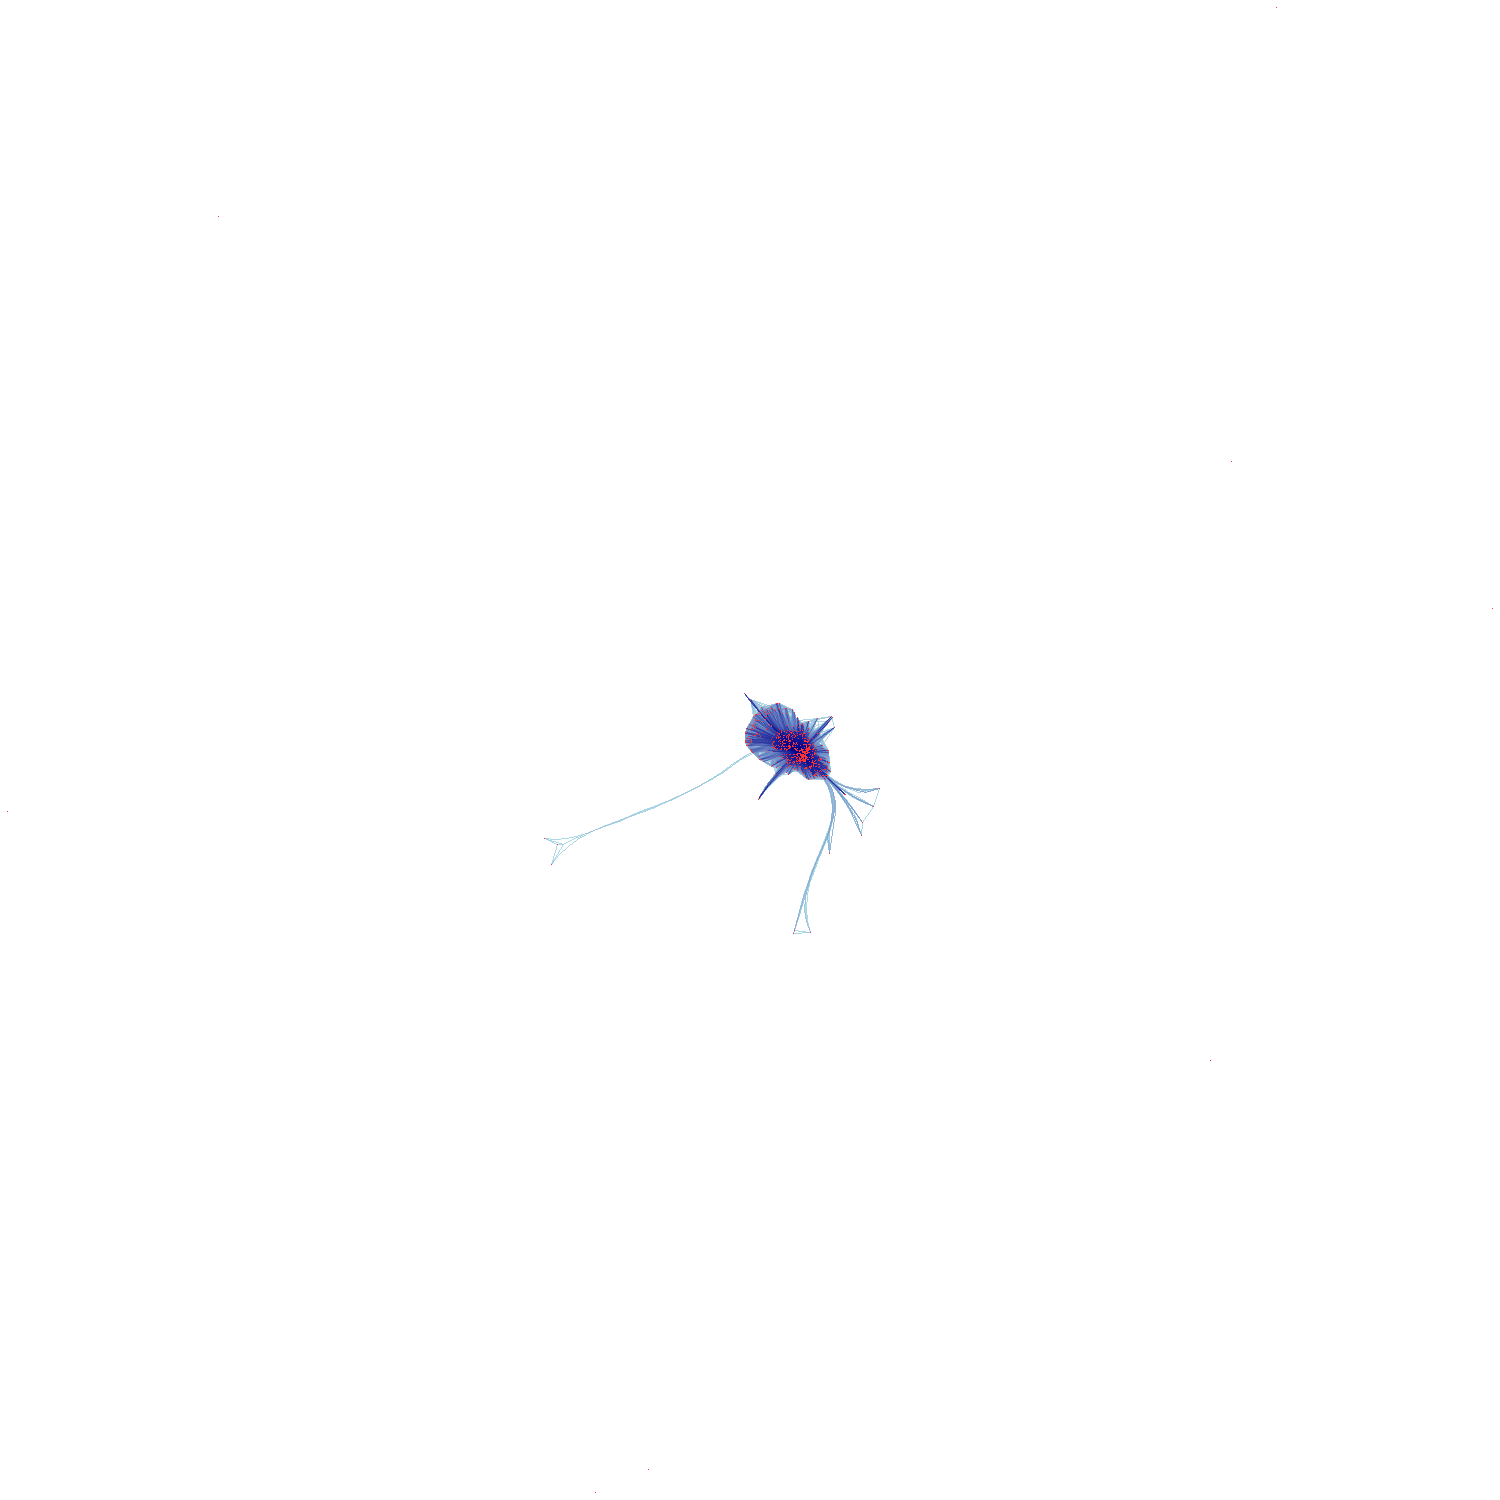
\includegraphics[width=.25\textwidth]{/files/src/.media/ego/grafo_forceatlas2_1.png}}\hfill
    \subfloat[$u = 2$]{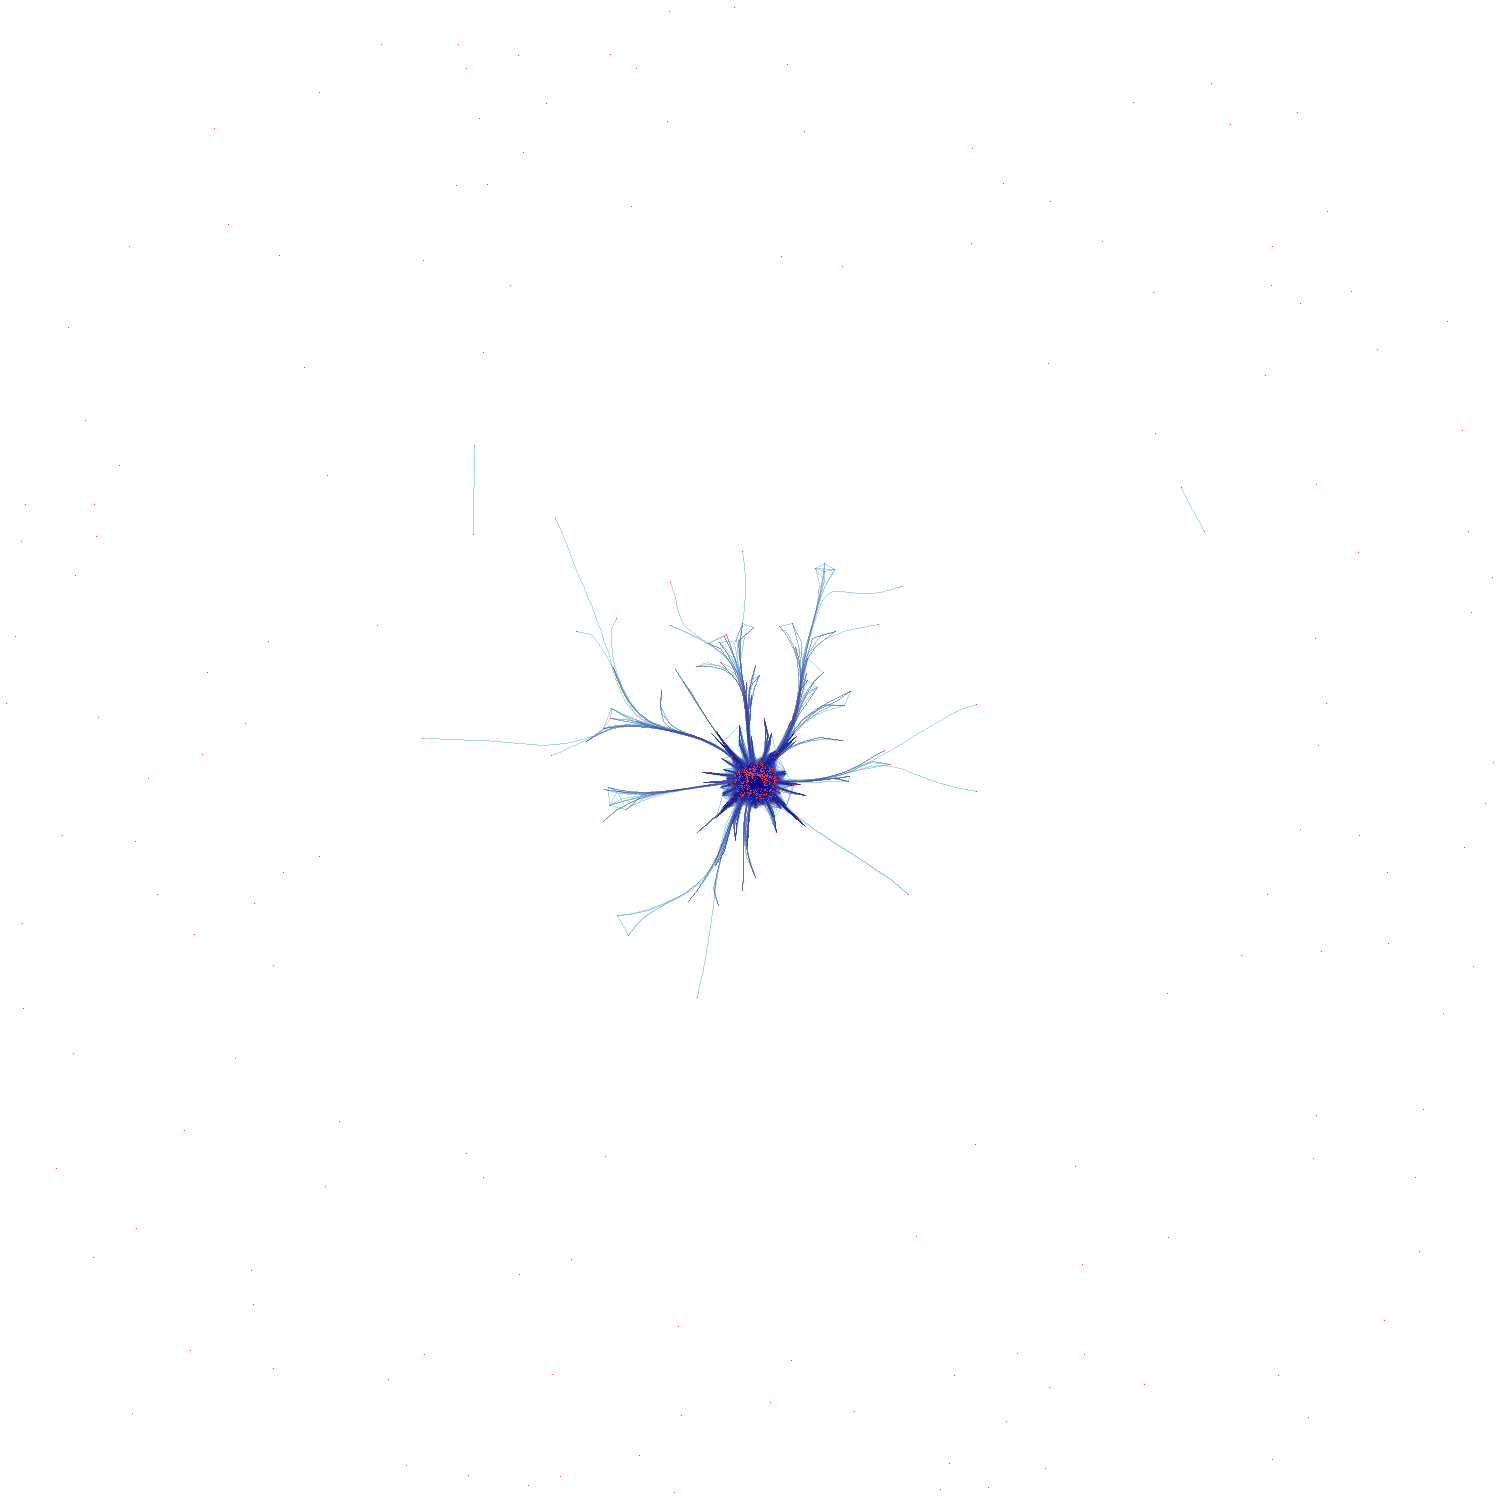
\includegraphics[width=.25\textwidth]{/files/src/.media/ego/grafo_forceatlas2_2.png}}\hfill
    \\[\smallskipamount]
    \subfloat[$u = 3$]{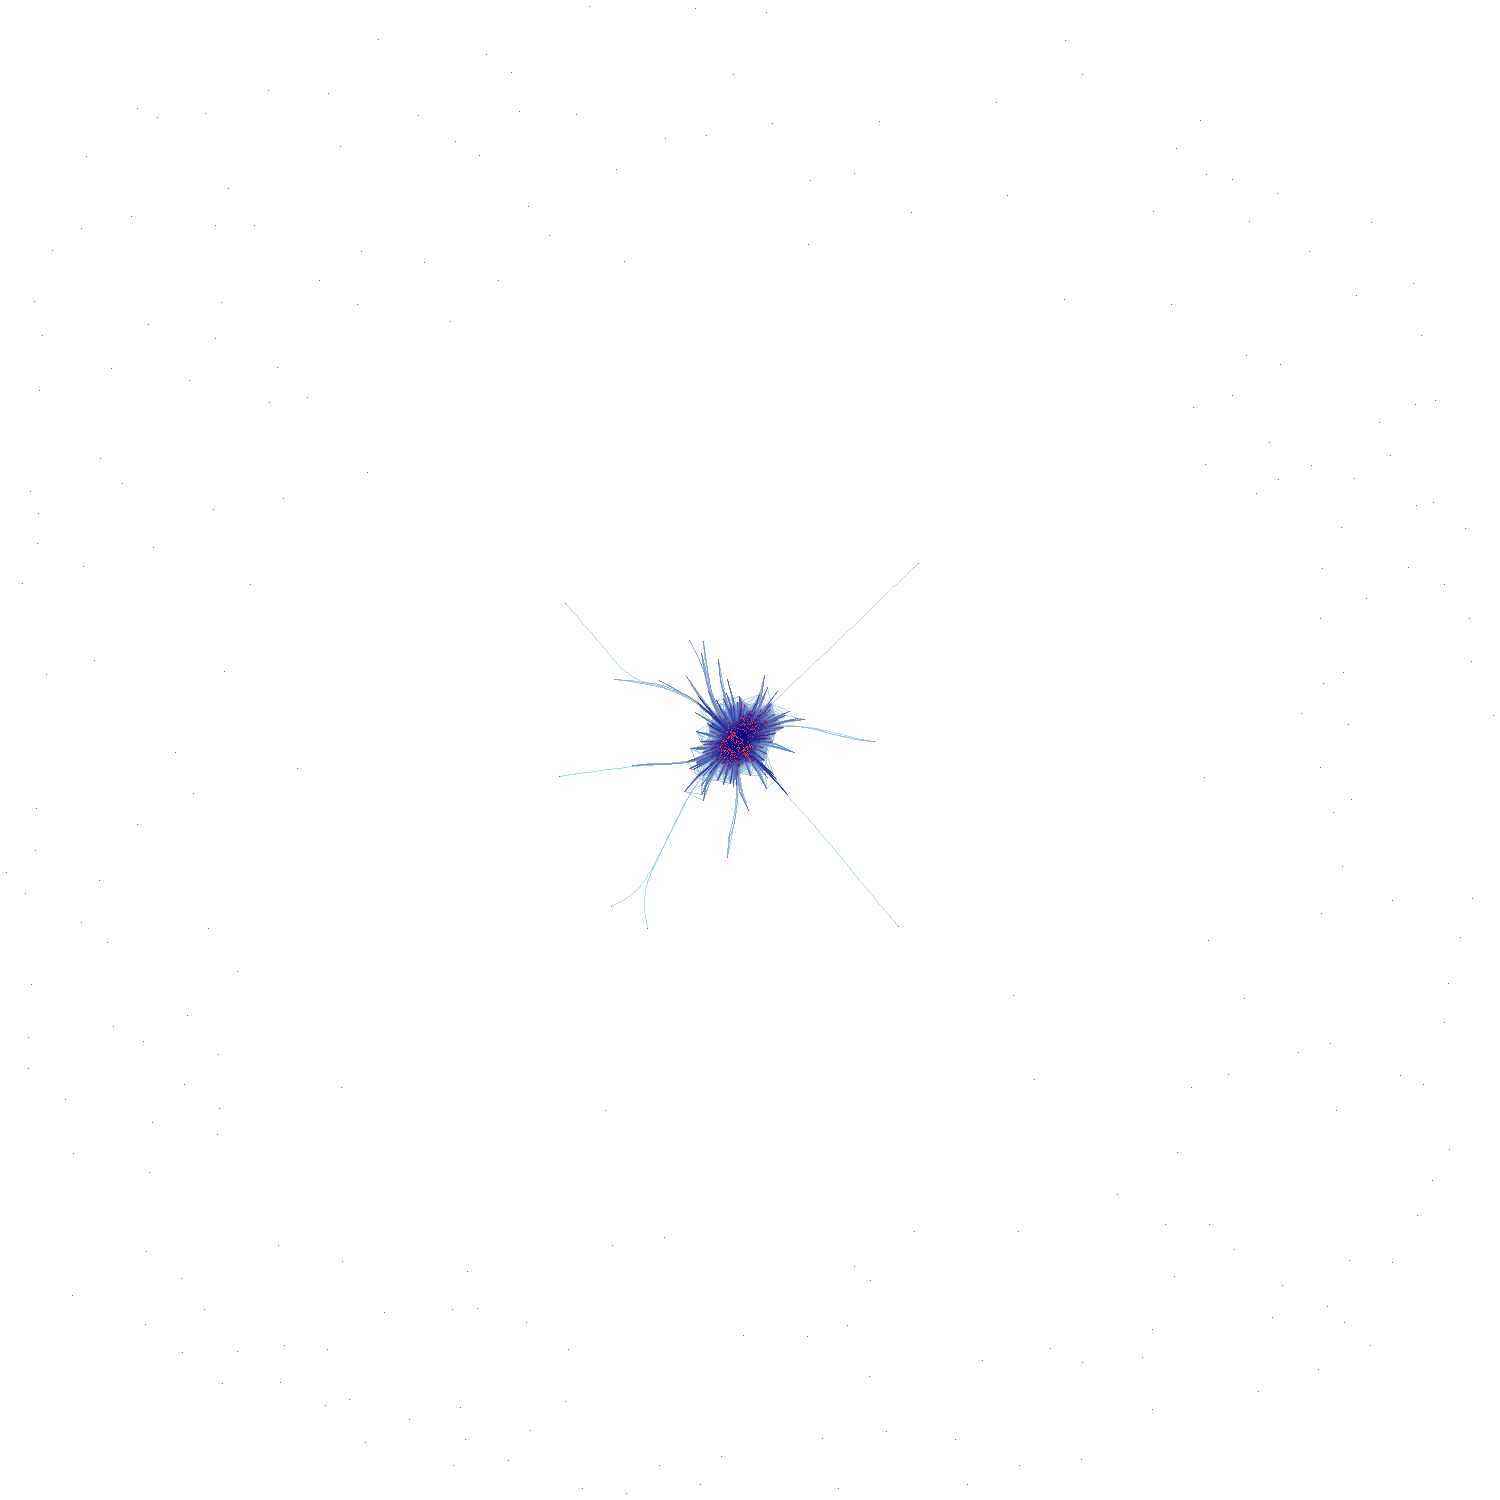
\includegraphics[width=.25\textwidth]{/files/src/.media/ego/grafo_forceatlas2_3.png}}\hfill
    \subfloat[$u = 4$]{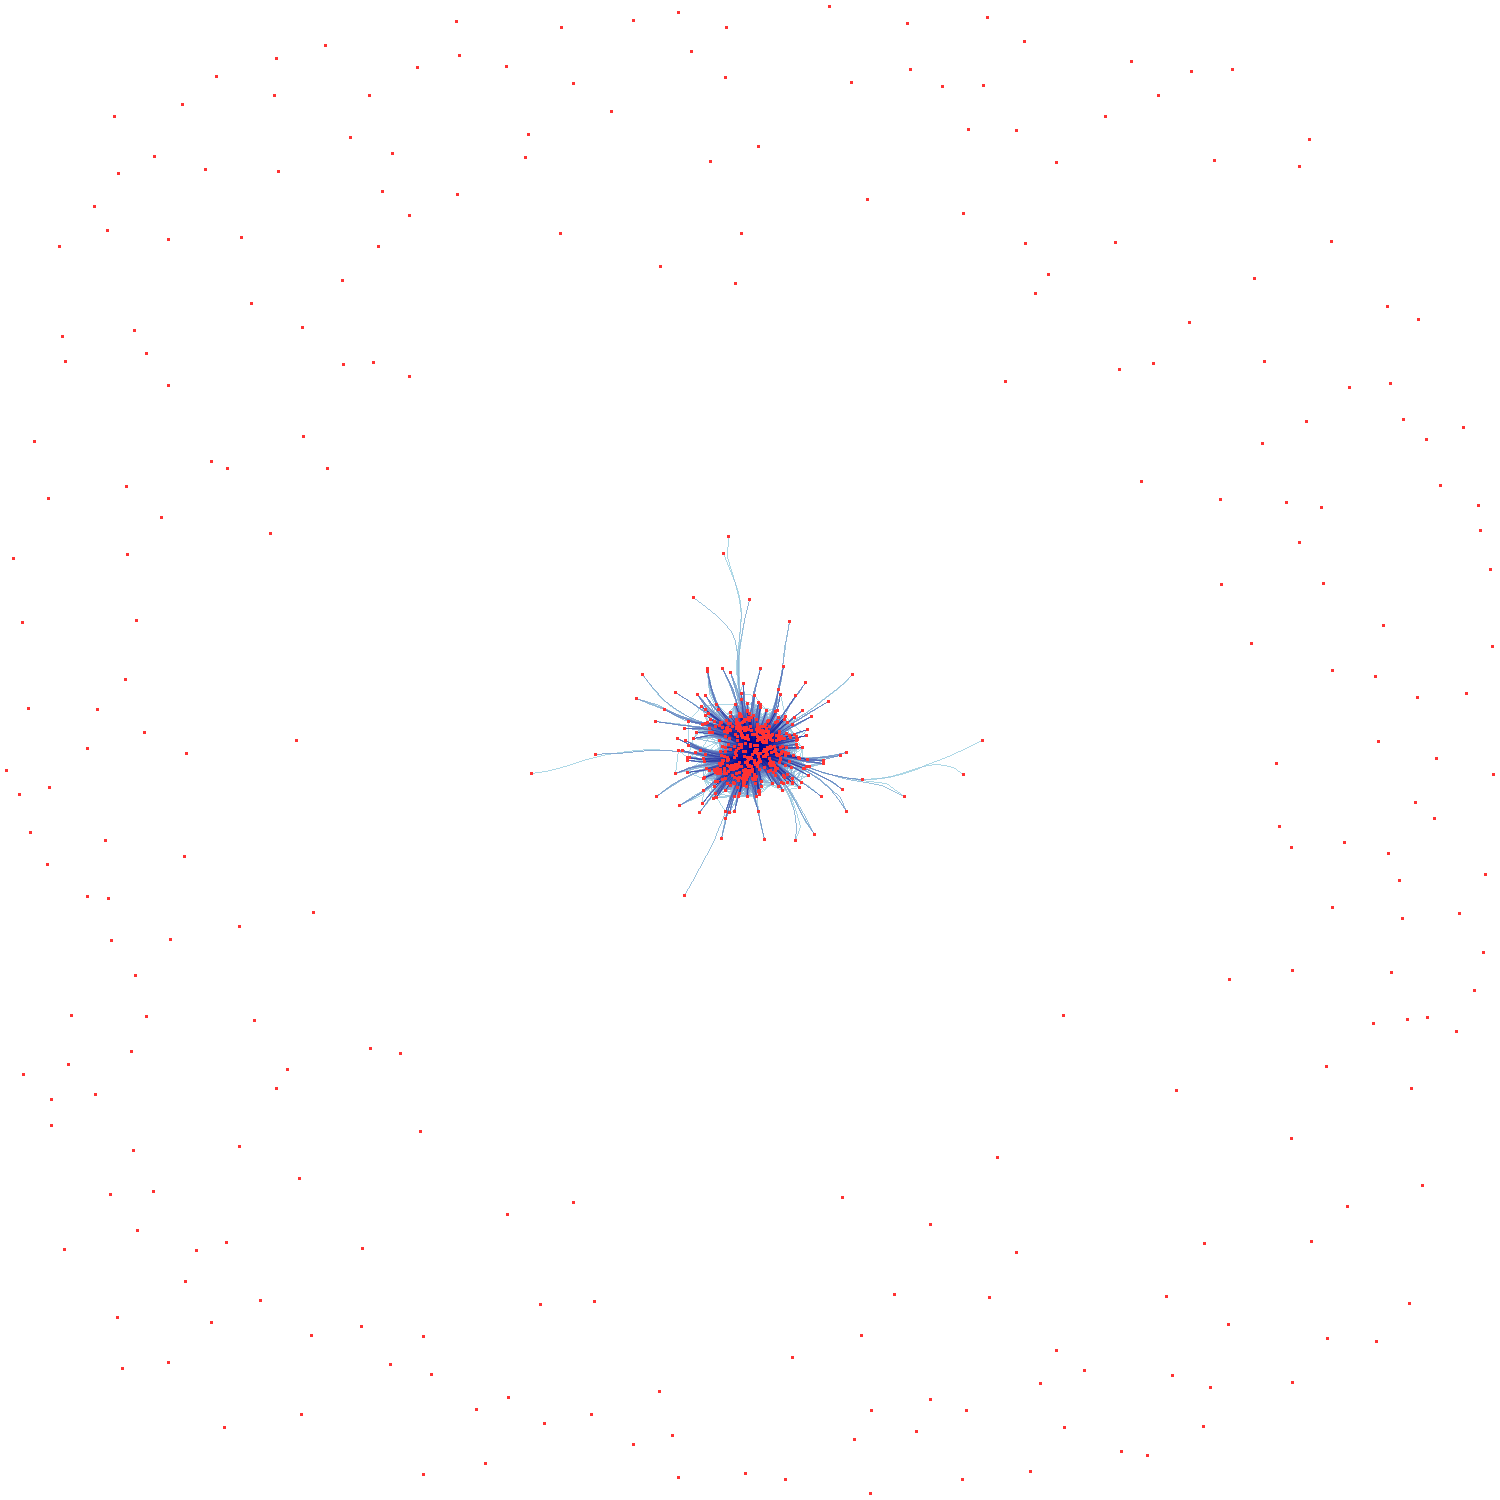
\includegraphics[width=.25\textwidth]{/files/src/.media/ego/grafo_forceatlas2_4.png}}\hfill
    \subfloat[$u = 5$]{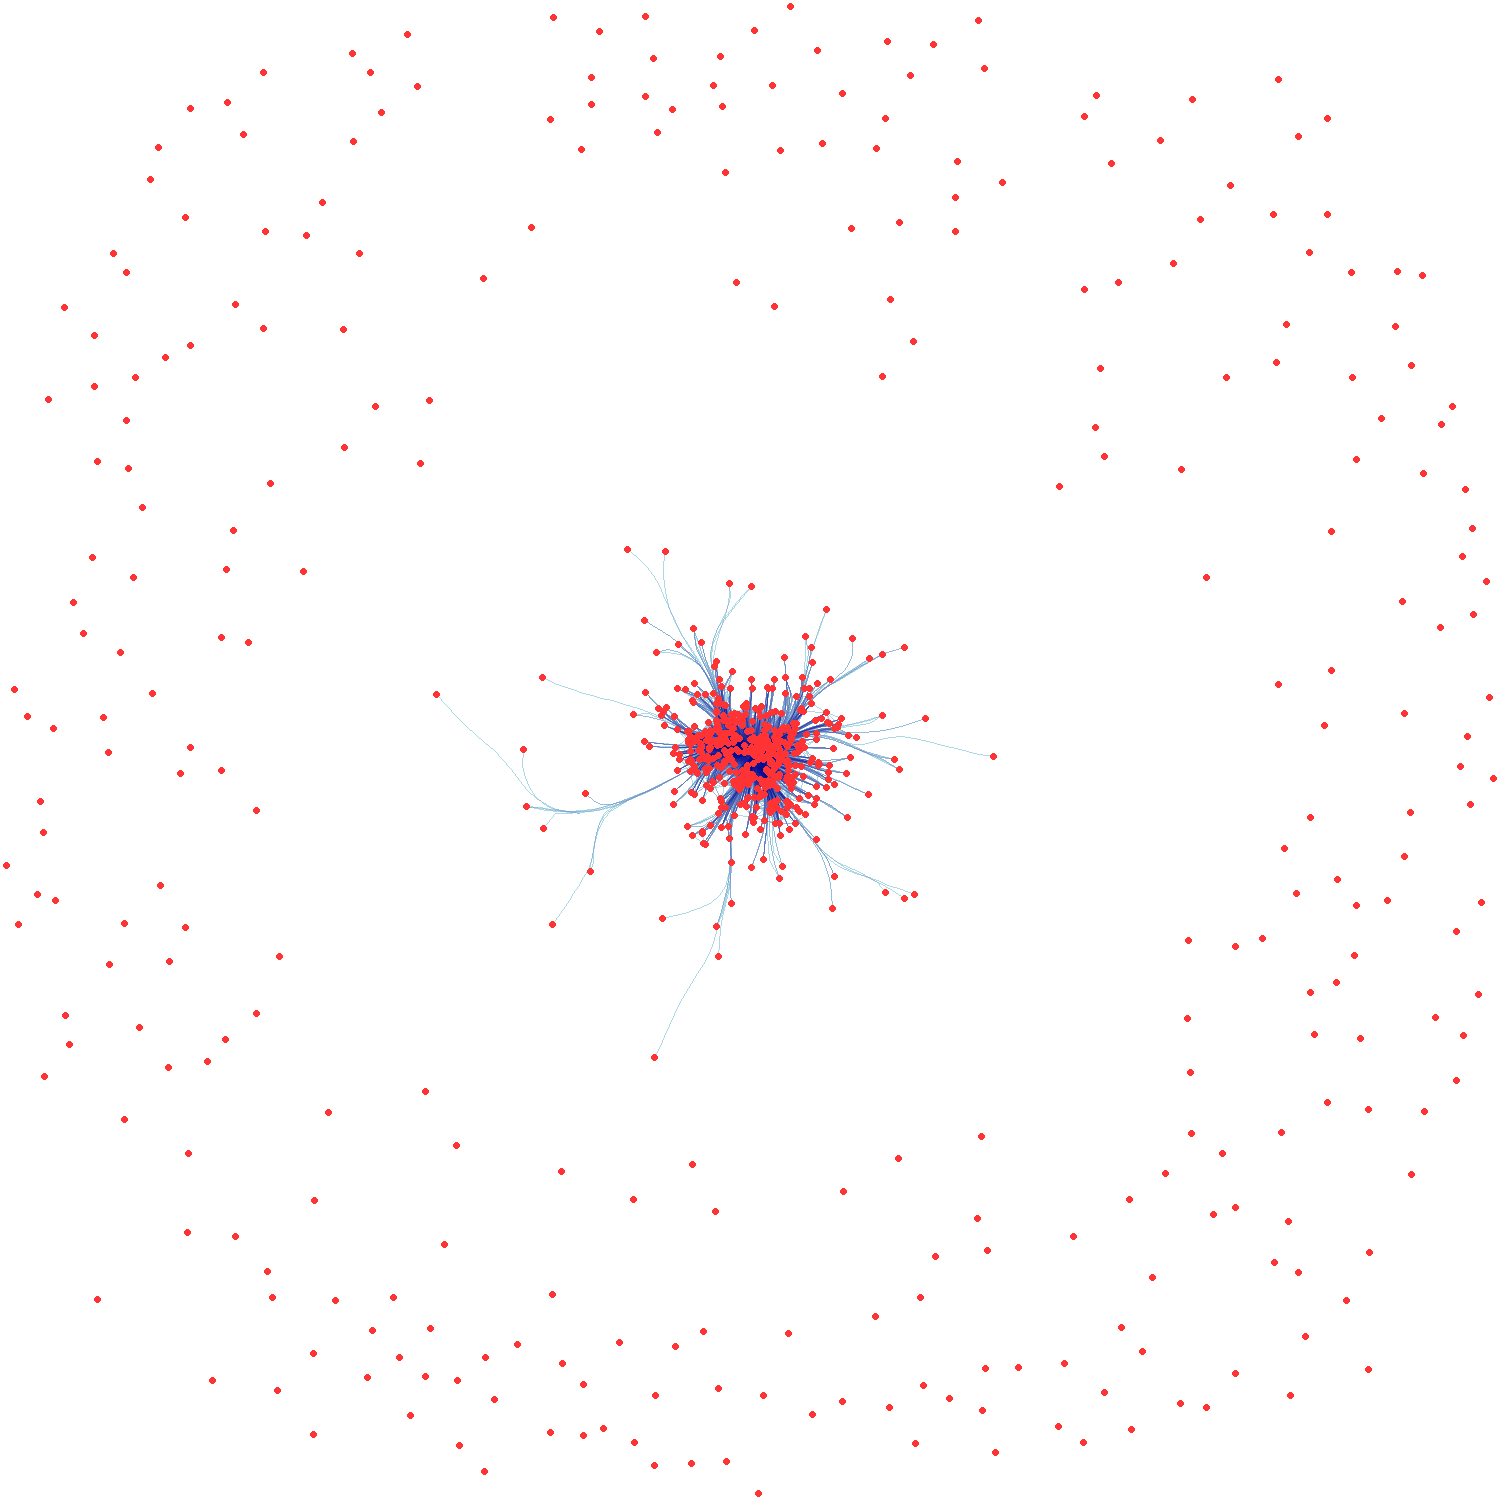
\includegraphics[width=.25\textwidth]{/files/src/.media/ego/grafo_forceatlas2_5.png}}\hfill
    \subfloat[$u = 6$]{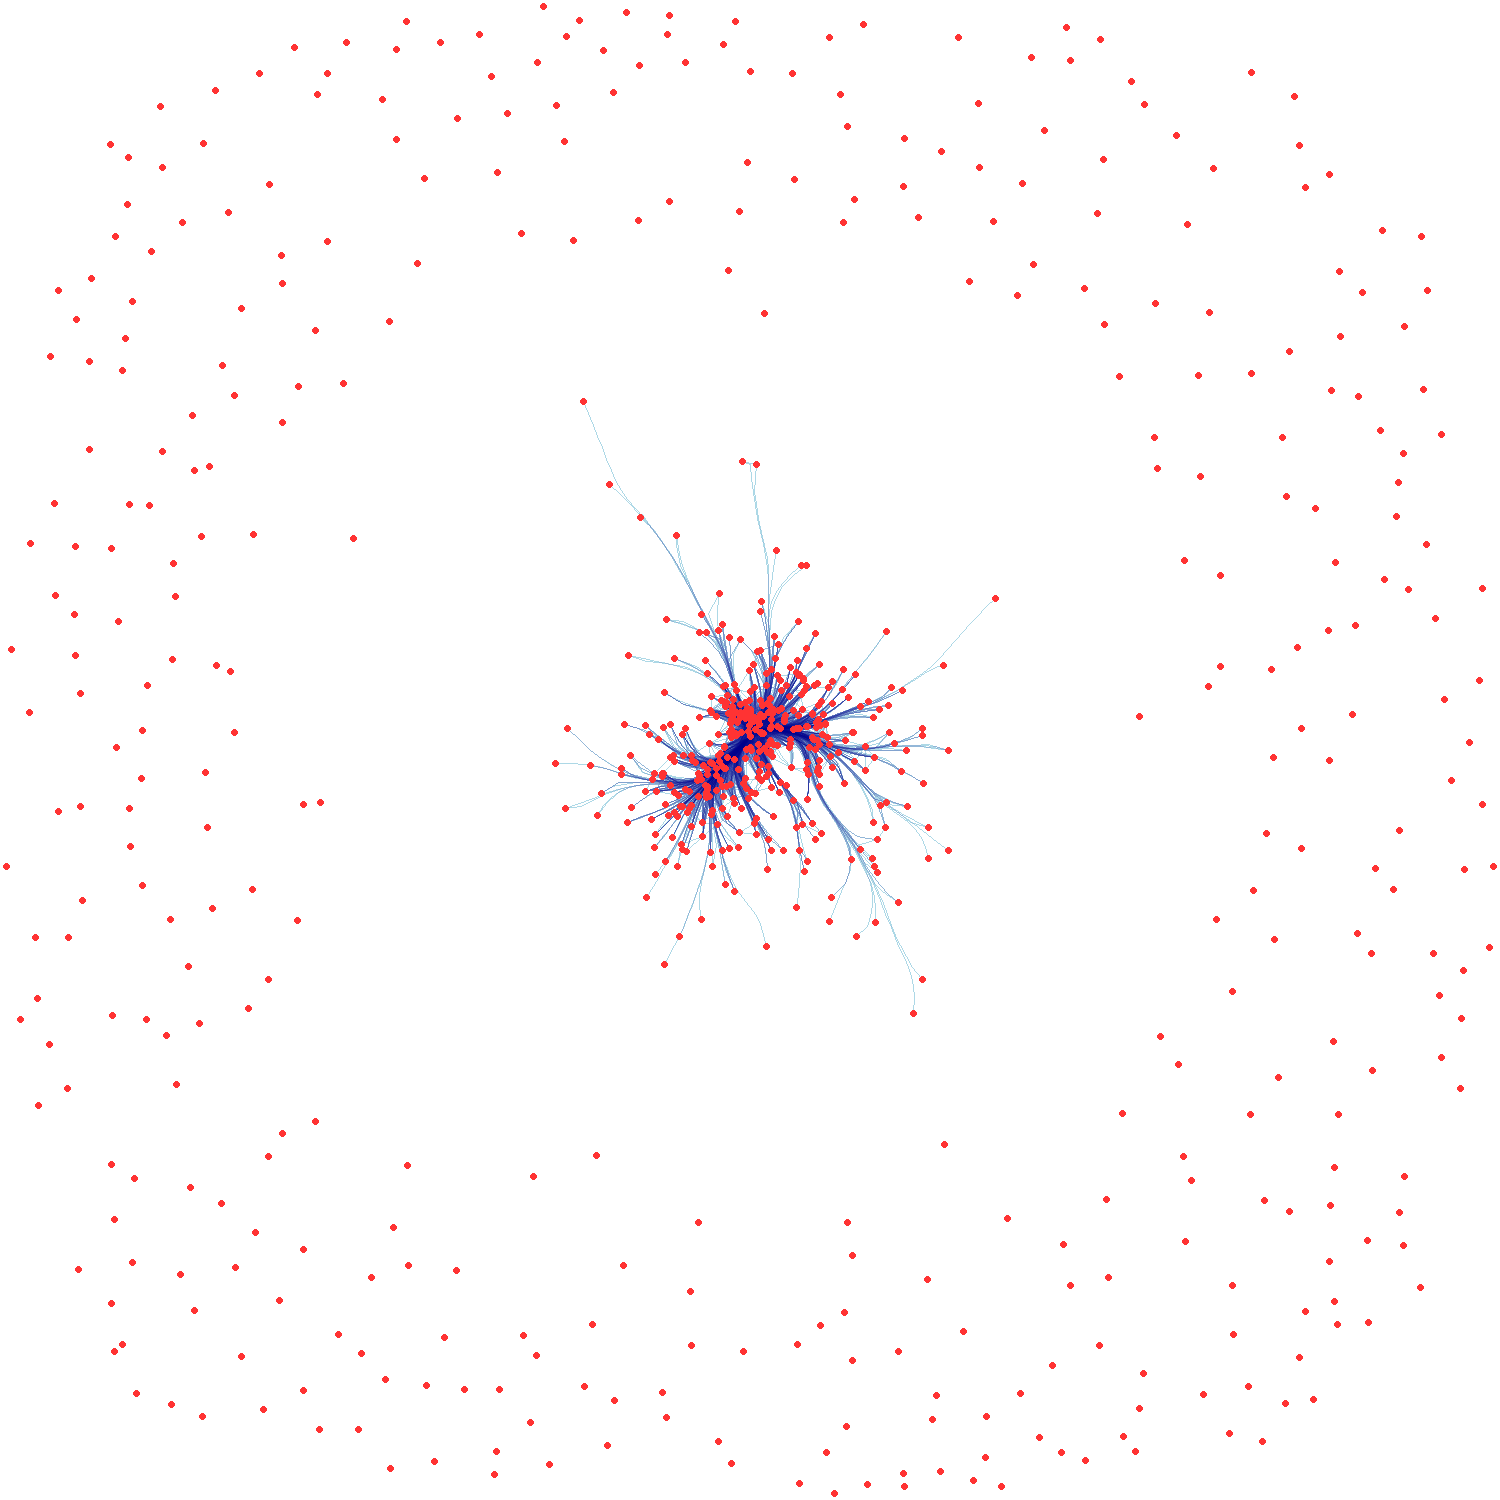
\includegraphics[width=.25\textwidth]{/files/src/.media/ego/grafo_forceatlas2_6.png}}\hfill
    \\[\smallskipamount]
    \subfloat[$u = 7$]{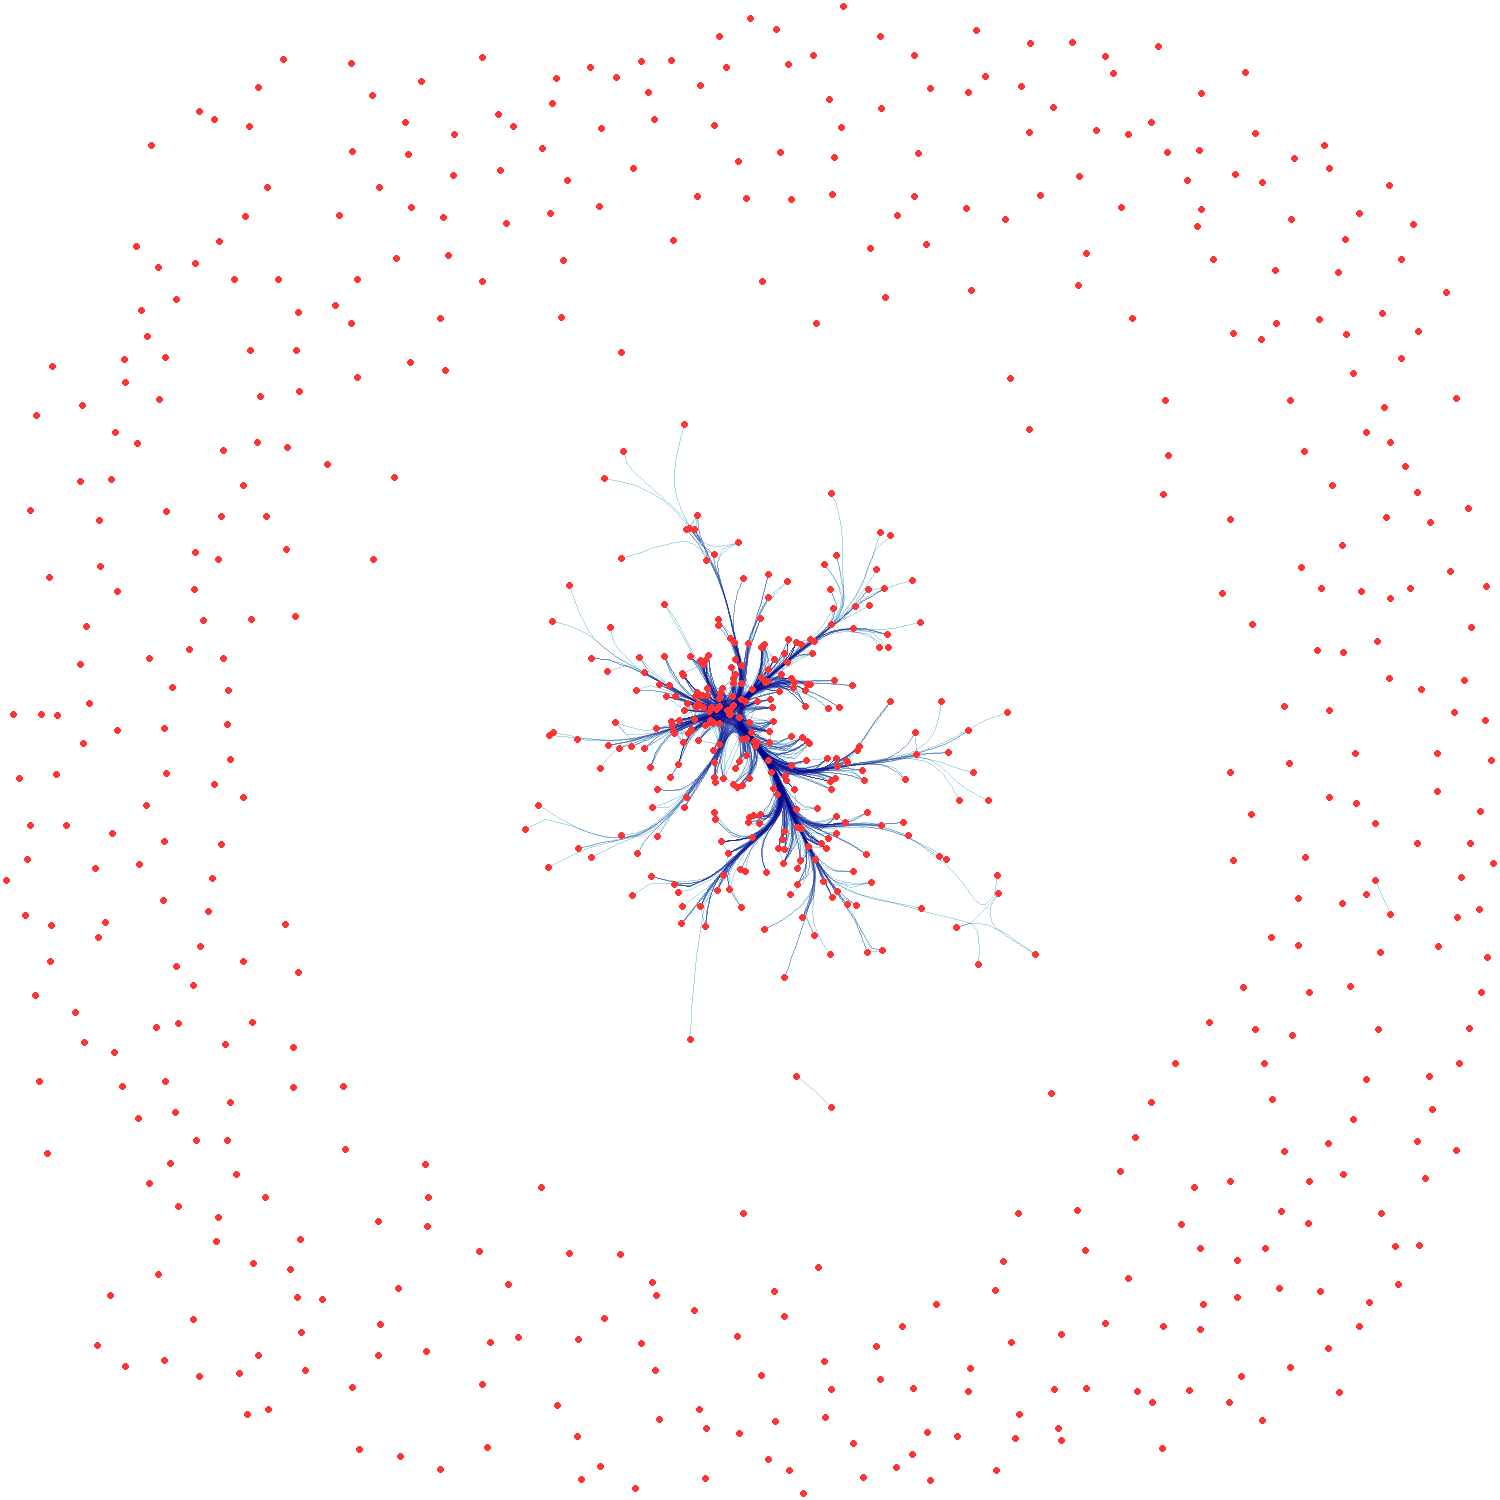
\includegraphics[width=.25\textwidth]{/files/src/.media/ego/grafo_forceatlas2_7.png}}\hfill    
    \subfloat[$u = 8$]{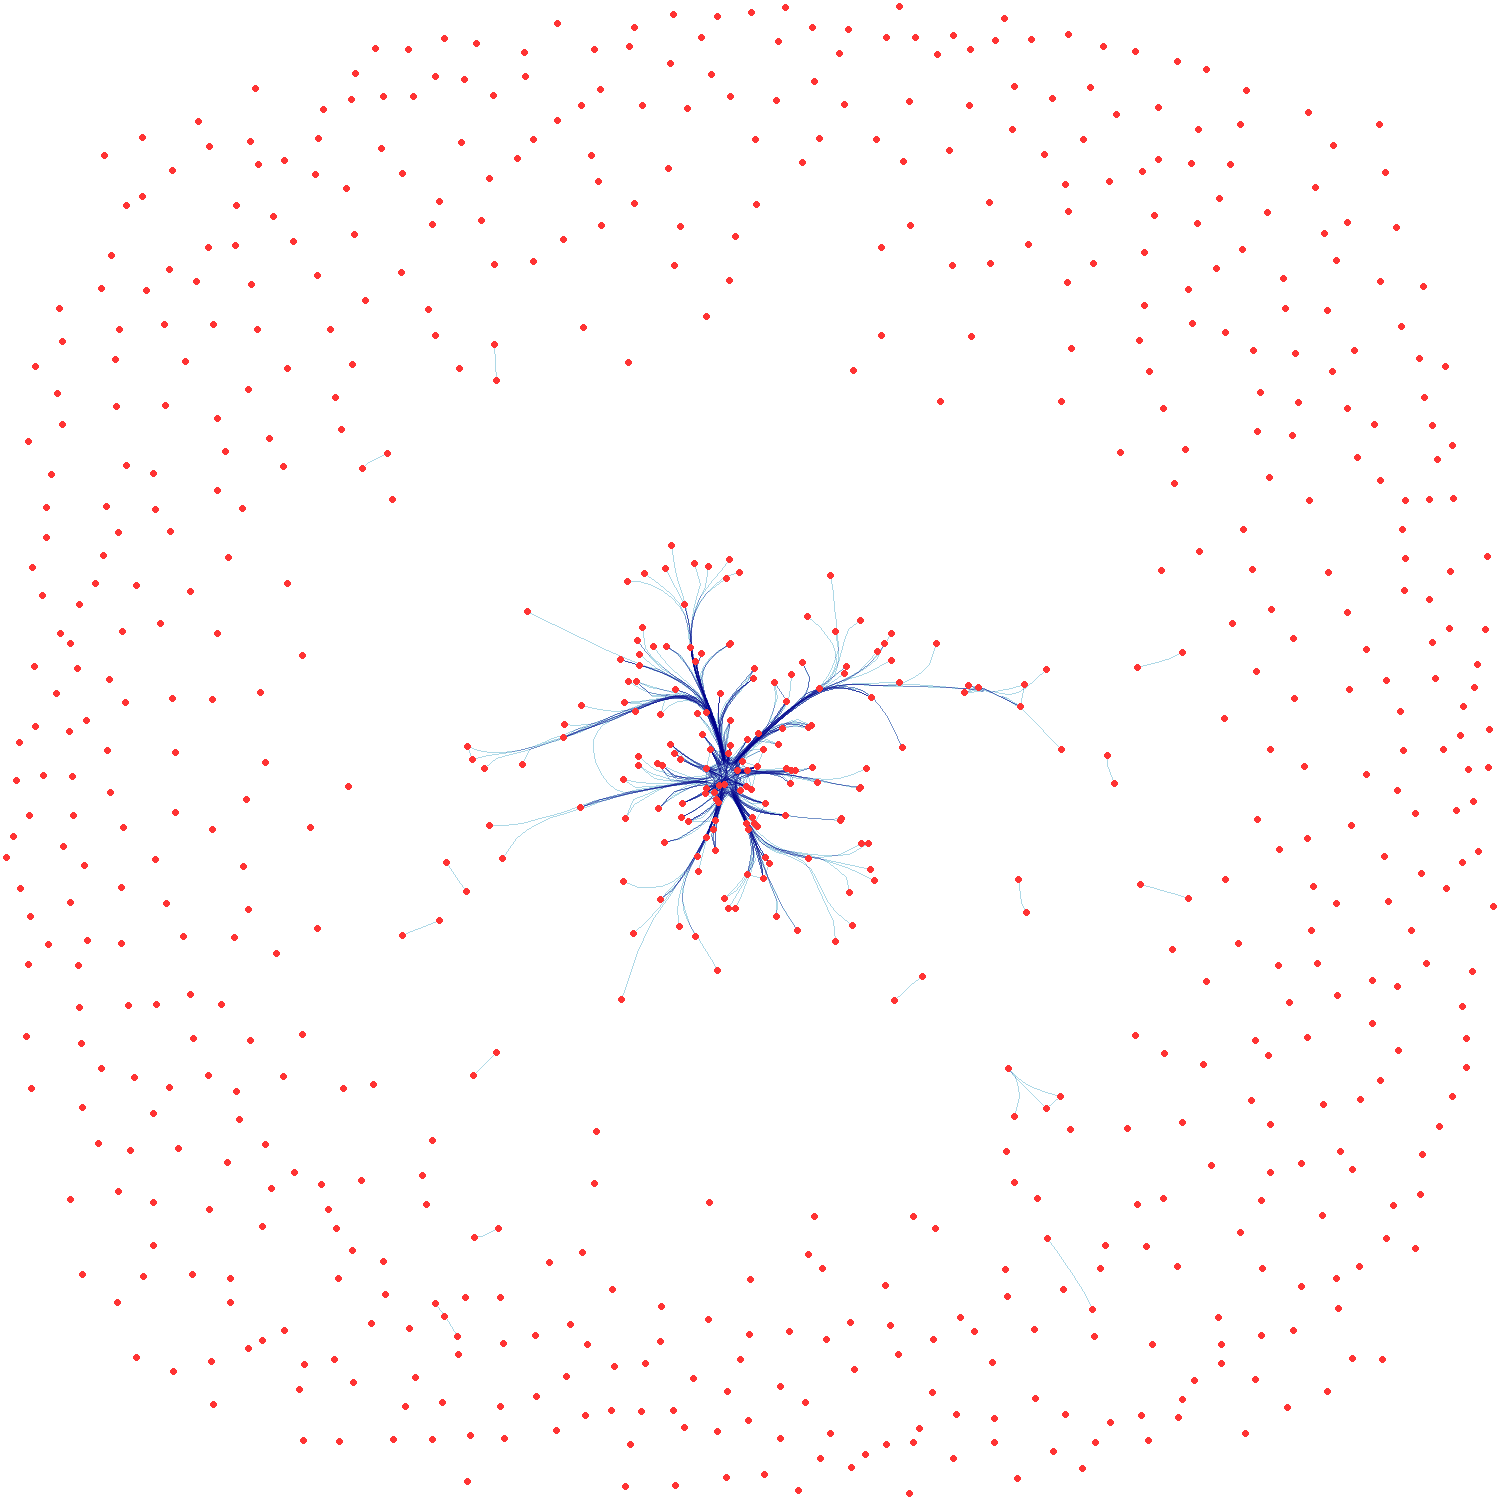
\includegraphics[width=.25\textwidth]{/files/src/.media/ego/grafo_forceatlas2_8.png}}\hfill
    \subfloat[$u = 9$]{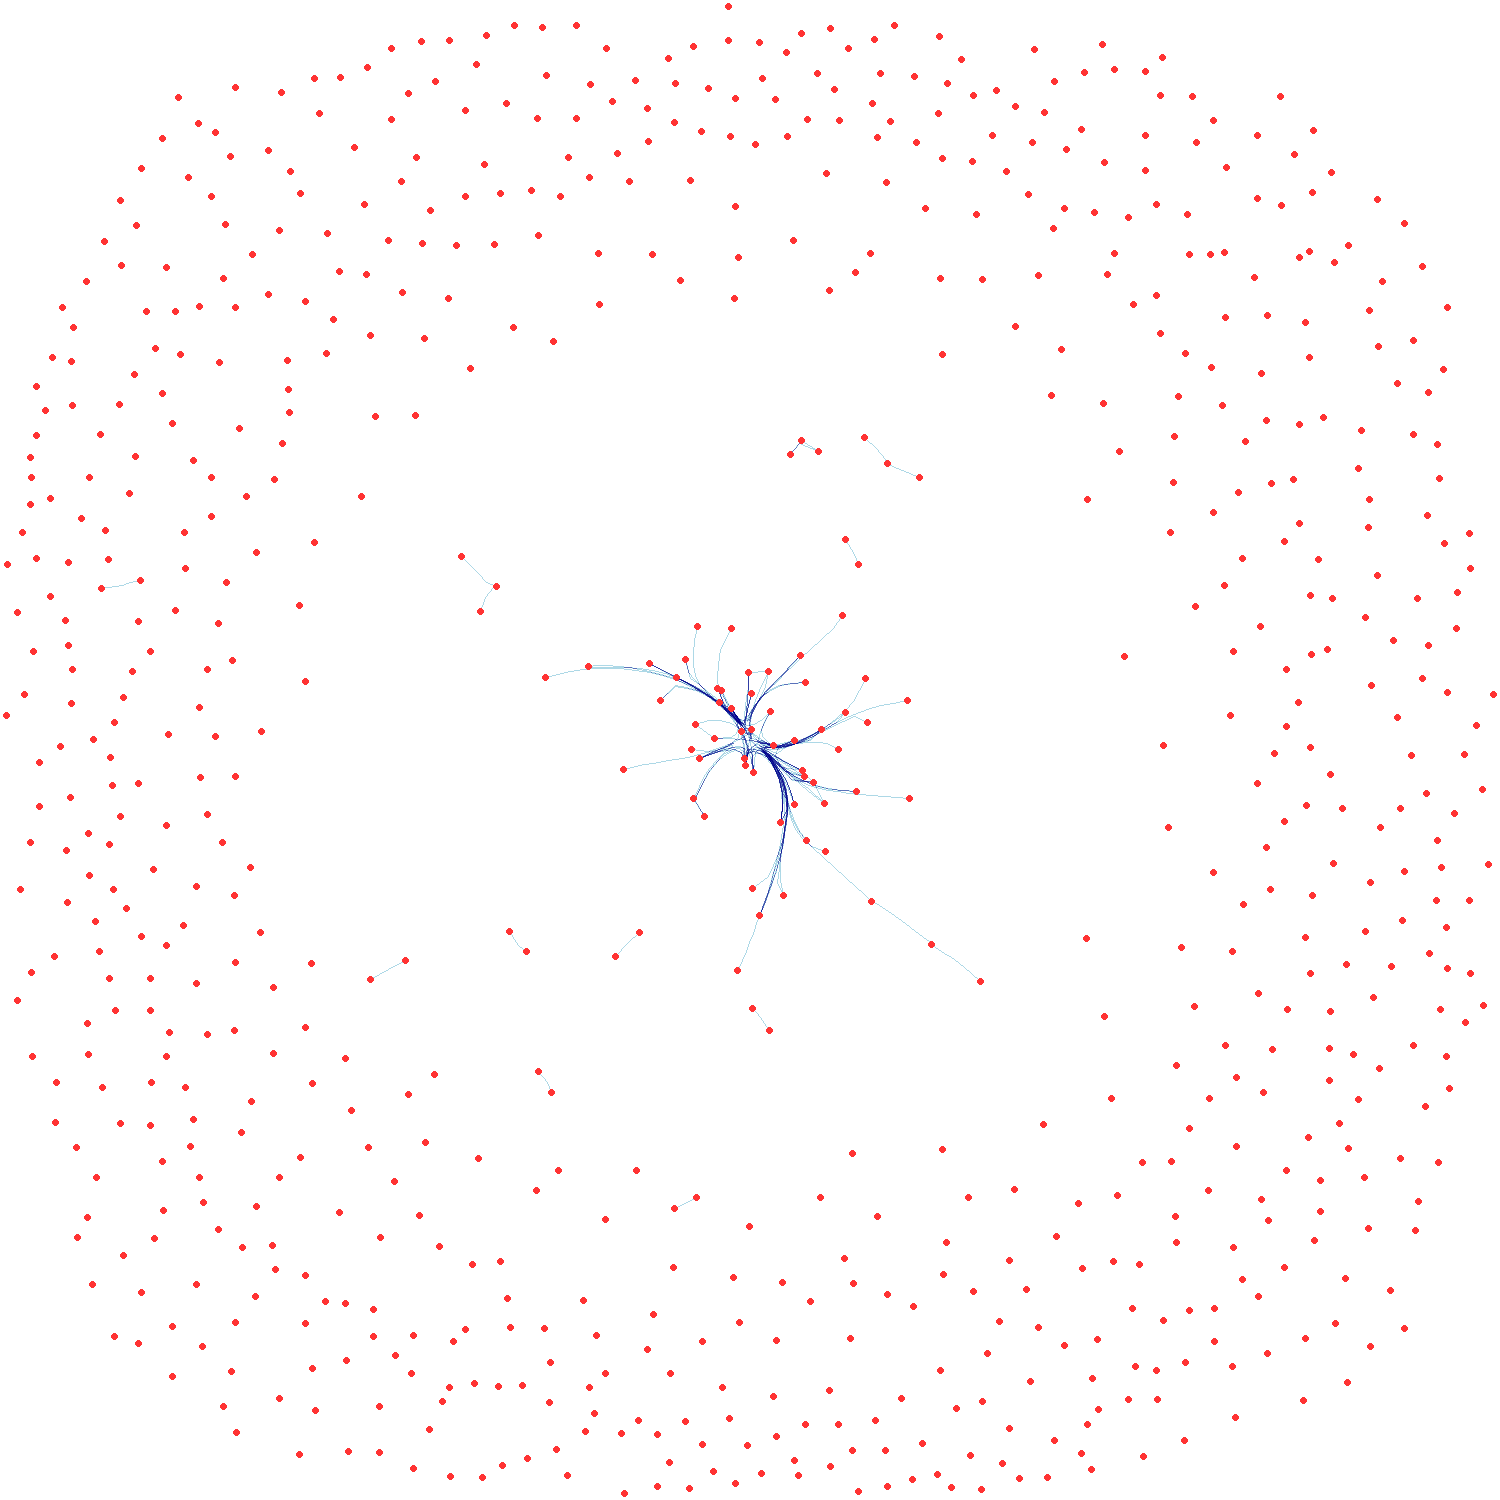
\includegraphics[width=.25\textwidth]{/files/src/.media/ego/grafo_forceatlas2_9.png}}\hfill
    \subfloat[$u = 10$]{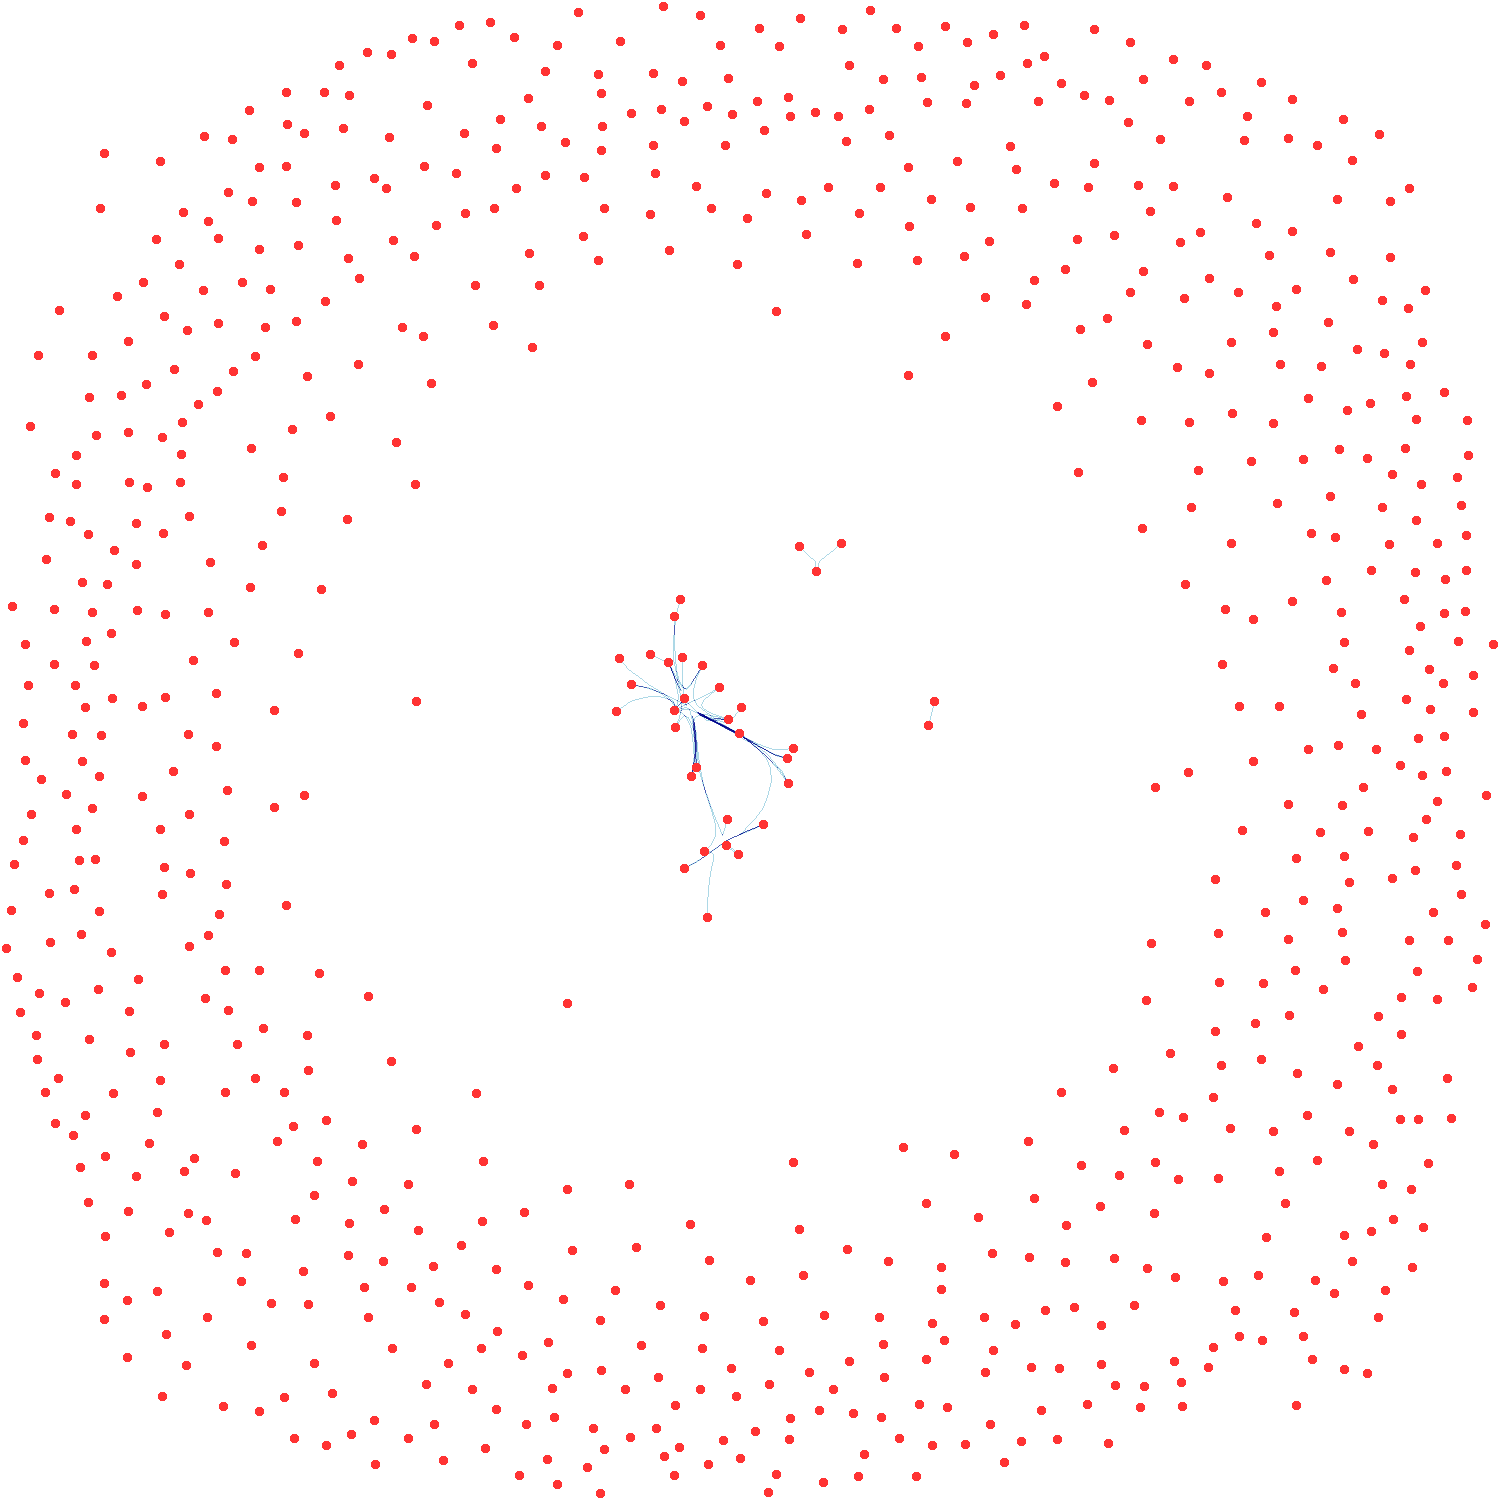
\includegraphics[width=.25\textwidth]{/files/src/.media/ego/grafo_forceatlas2_10.png}}\hfill
    \\[\smallskipamount]
    \subfloat[$u = 11$]{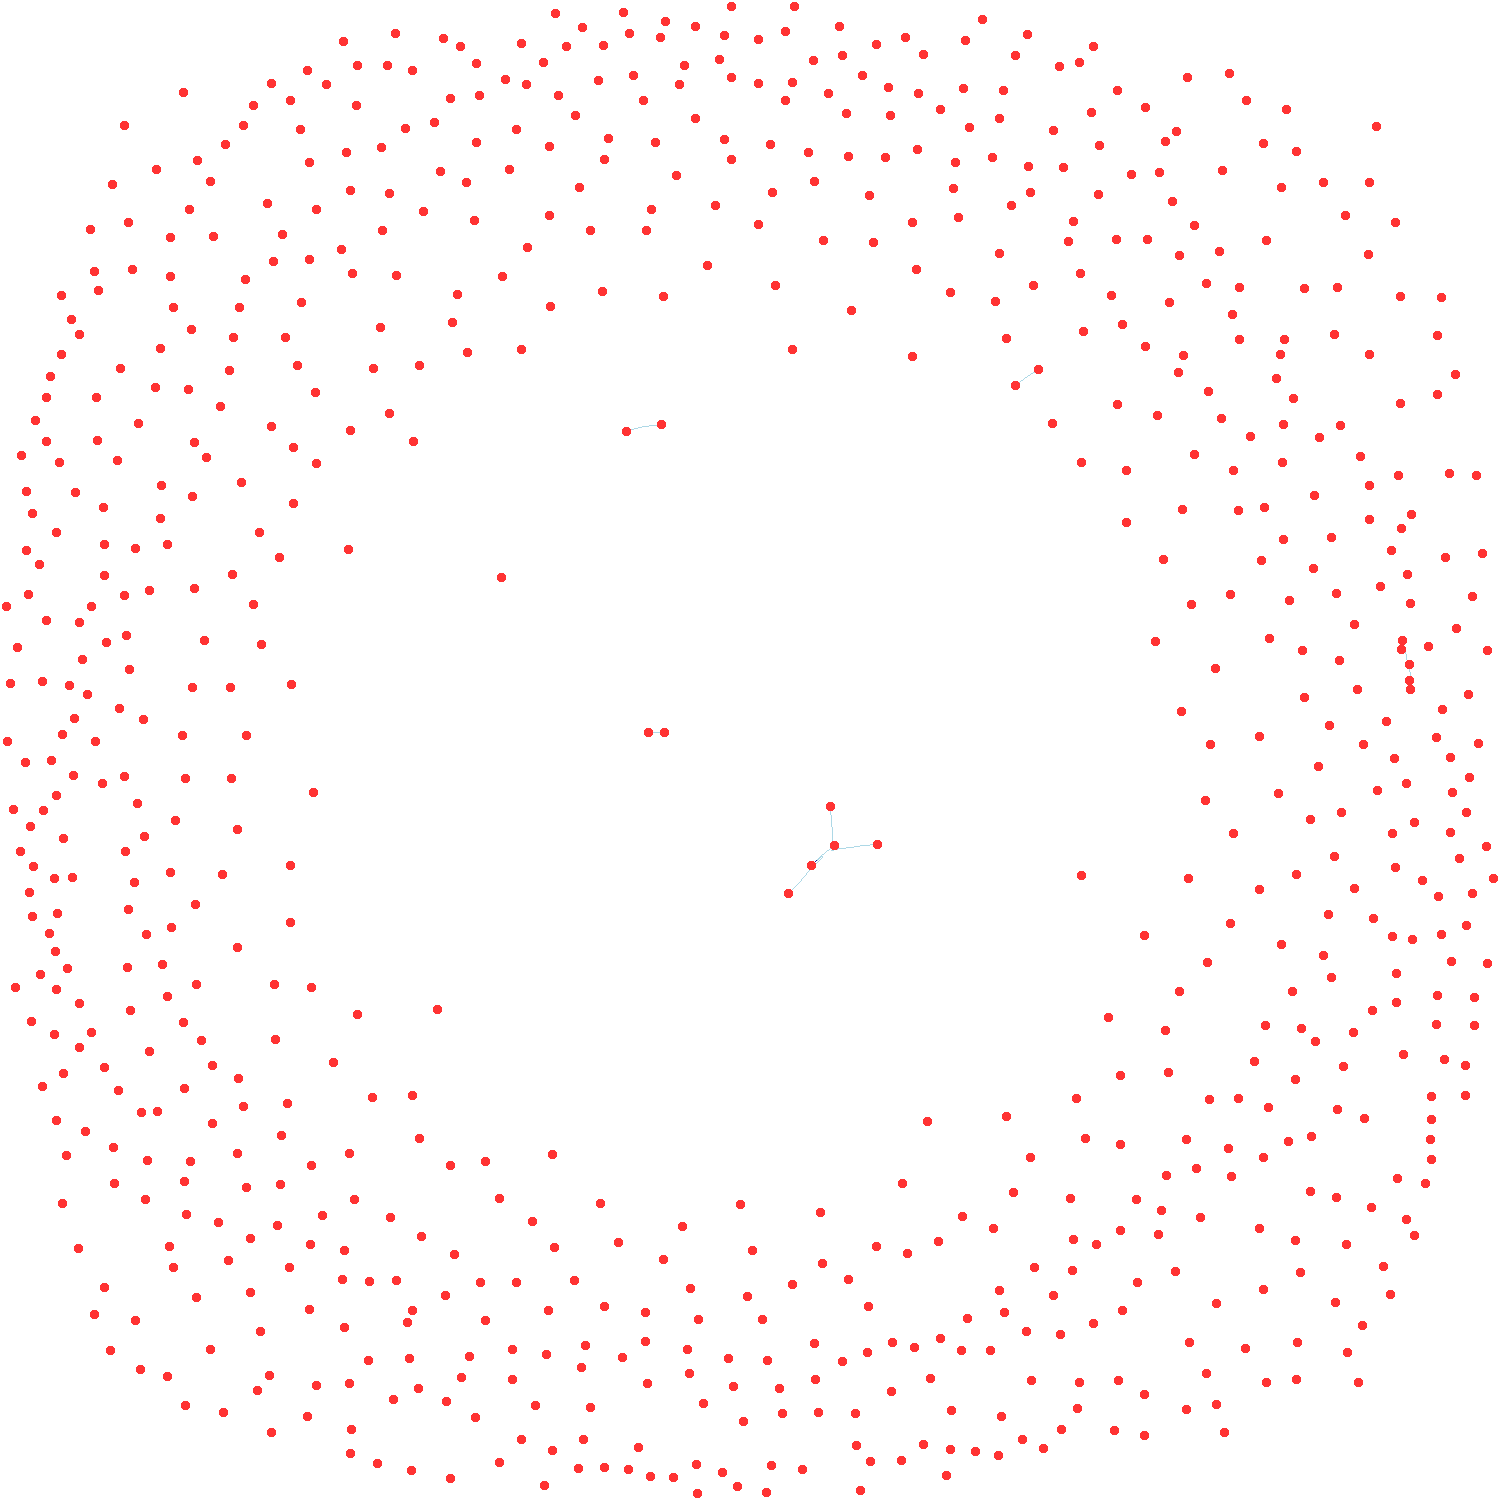
\includegraphics[width=.25\textwidth]{/files/src/.media/ego/grafo_forceatlas2_11.png}}\hfill
    \subfloat[$u = 12$]{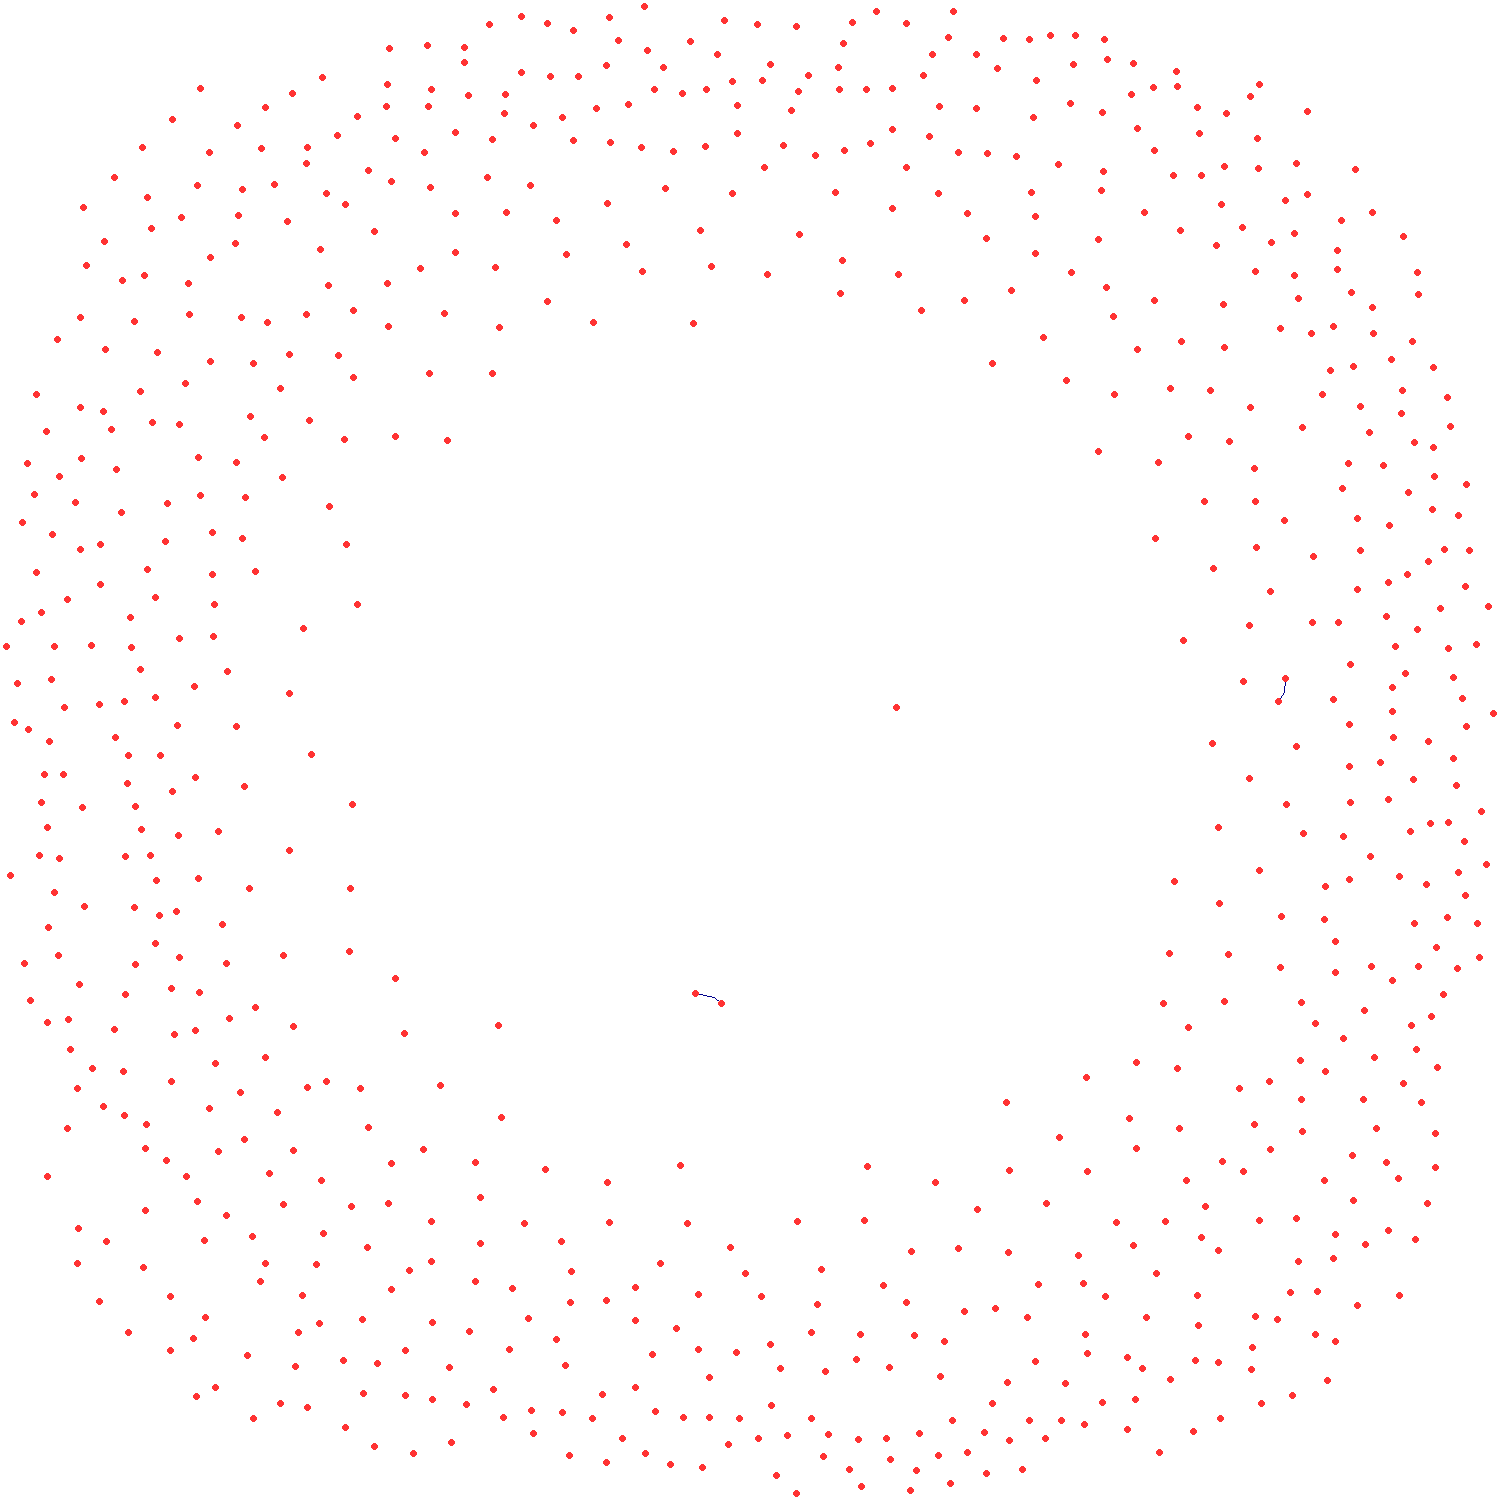
\includegraphics[width=.25\textwidth]{/files/src/.media/ego/grafo_forceatlas2_12.png}}\hfill
    \caption{Todos los grafos correspondientes a los diferentes umbrales, tomados para la matriz de similaridad de los atributos \textbf{C}. Observar que al aumentar $u$ crece la cantidad de nodos aislados.}
\end{figure}

\vspace{1em}


% === COMPARACION === %

\vspace{2em}
\subsection{Comparación con la red original}

Nos encontramos con diferentes grafos construidos en base a los atributos en \textbf{C}. Buscamos ahora comparar nuestras aproximaciones con la red original. 
Un primer acercamiento a este problema fue calcular la cantidad de posiciones coincidentes entre las matrices de adyacencia y dividir por los elementos totales. La lógica por detrás del método es que nuestros grafos serán más similares entre sí por cada conexión y `no conexión' acertada. Entonces, por cada 0 y 1 coincidente en nuestra aproximación y \textbf{E} nos acercaríamos más a un 100\% de similitud. 

\begin{figure}[!htbp]
\begin{equation*}
    \begin{bmatrix}
    0  &\%\ 7.6054231   \\
    1  &\%\ 32.947445   \\
    2  &\%\ 58.570142   \\
    3  &\%\ 70.993985   \\
    4  &\%\ 84.162733   \\
    5  &\%\ 91.537012   \\
    6  &\%\ 94.322073   \\
    7  &\%\ 95.214277   \\
    8  &\%\ 95.403337   \\
    9  &\%\ 95.446393   \\
    10 &\%\ 95.455457   \\
    11 &\%\ 95.458695   \\  
    12 &\%\ 95.459342   \\
    13 &\%\ 95.459990   \\
    \end{bmatrix}
\end{equation*}
\caption{Similitud elemento a elemento de las matrices de adyacencia, la primer columna representa el umbral tomado para la aproximación y la segunda el porcentaje de elementos correctamente estimados con respecto a la original. Se incluye un grafo sin aristas, con $u = 13$.} \label{promedio_similaridad}
\end{figure}

Como puede observarse, desafortunadamente, los grafos con muy pocas conexiones, como prueban ser tomando los umbrales $u > 10$, tienen de los valores más altos, mientras que otros con cantidad de aristas similares a la red original, como con $u = 5$ o $u = 6$ (16.850 y 5.727 conexiones respectivamente), parecerían ser peores aproximaciones. Esto se da por la naturaleza rala de nuestras matrices de adyacencia. La de la red `ego' \textbf{E} es de $786 \times 786$, con 617.796 elementos, y tan solo 28.048 (\% 4.54) de ellos son no nulos. Es decir, es rala en un \% 95.46. Es por esto que comparar elemento a elemento no prueba ser un método muy descriptivo de qué tan buena es una aproximación, ya que cualquiera con pocos elementos coincidirá en un $\sim$\% 95.

\vspace{1em}

Empleamos entonces otros dos métodos de comparación: \textit{la correlación de las matrices de adyacencia estiradas} y \textit{la correlación de las listas de autovalores}. La correlación es una covarianza normalizada con valores en (-1, 1), donde números mayores indican una mayor similitud. Esta es descrita por la siguiente fórmula:

\begin{equation}
    Corr(x, y) = \frac{(x - \mu_{x}) \cdot (y - \mu_{y})}{\sqrt[]{(x - \mu_{x})^{2} \cdot (y - \mu_{y})^{2}}}
\end{equation}

siendo $\mu$ el valor medio de los vectores.

\vspace{1em}
\begin{figure}[!htbp]
\centering
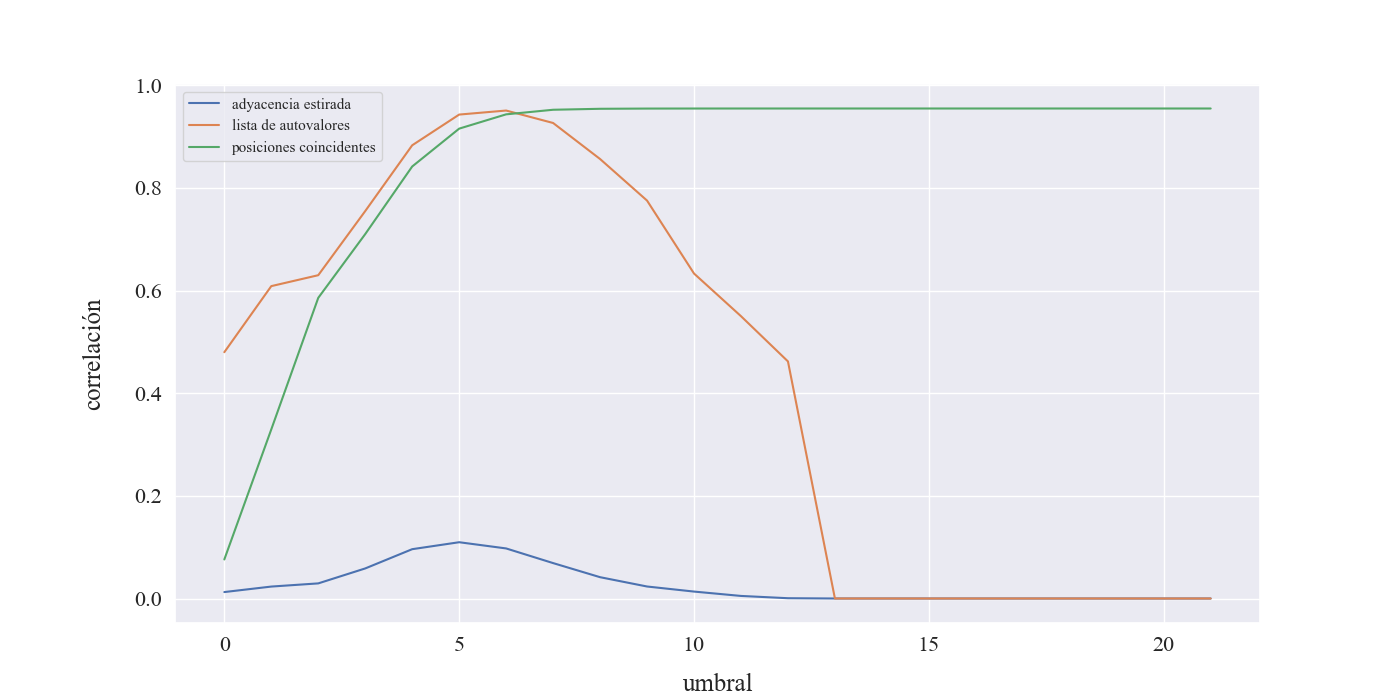
\includegraphics[scale=0.45]{/files/src/.media/ego/facebook_similaridad.png}
\caption{Correlaciones entre matrices de adyacencia y listas de autovalores según los diferentes umbrales.}
\label{grafo_correlaciones}
\end{figure}

En la figura (\ref{grafo_correlaciones}.) se puede apreciar que se obtienen resultados considerablemente diferentes a los de nuestro primer método de comparación. En un primer lugar, siguiéndonos de la correlación entre las matrices de adyacencia, parecería que las mejores aproximaciones son las de cantidad de aristas similares a la red original, con los umbrales $u \in [4,7]$, mientras que los grafos vacíos con umbrales más altos pasan a tener correlación 0. De la misma forma, analizando con los autovalores se obtienen resultados similares, donde la mayor correlación se halla con los umbrales de valores medios.  


% === OPTIMIZACION === %

\vspace{2em}
\subsection{Optimización}




% === PCA === %

\vspace{2em}
\subsection{PCA}

\newpage

% conclusiones
\section{Conclusiones}
\vspace{2em}

En este trabajo, habiendo implementado el método de la potencia y experimentado con él, observamos distintos problemas en el mismo, tales como el error numérico o su incapacidad de calcular los autovectores de las matrices con autovalores repetidos en valor absoluto. Es por esto que experimentamos con diferentes modificaciones al método propuesto para abarcar todos los casos posibles. Además, propusimos optimizaciones al algoritmo, como lo es ir de a pasos pares, para acortar la cantidad de iteraciones que requería para converger. 

\vspace{1em}
Luego, con la implementación del método, comenzamos a experimentar con distintos casos de uso práctico. Por un lado, en el apartado del \textit{Club de Karate}, vimos la utilidad de la centralidad de autovector y conectividad algebraica en la matriz laplaciana para evaluar las distintas características de una red. 

\vspace{1em}
Por otro lado, el análisis de las red `Ego' de Facebook nos permitió experimentar con diferentes aproximaciones de las mismas, evaluando sus similitudes a la original y determinando cuáles fueron las mejores. También, recurrimos al análisis de componentes principales (PCA) para reducir la dimensionalidad del conjunto de datos, y observamos los resultados sobre distintos rangos de la matriz de covarianza. Afirmamos de esta manera la posibilidad de aplicar una reducción, a bajo costo de calidad en nuestra predicción.

\vspace{1em}
En conclusión, observamos que el cálculo de autovalores y autovectores no es una tarea sencilla, pero a su vez posee una gran utilidad para el estudio de matrices. Nos brindan información de la estructura subayacente de los datos y su comportamiento, por lo que son imprescindibles para el análisis de toda clase de problemas.

\newpage

% apendice
\section{Apéndice}

\vspace{1em}
\begin{figure}[!htbp]
    \scalebox{0.7}{
        \begin{tabular}{ |c|c|c|c|c|c|c| } 
        \hline
        p & atributos & u & conexiones & coincidentes & adyacencia estirada & autovalores \\
        \hline
        0.5             &12             &0            &229,602                 & 28.19\%\     & 1.73\%\               & 58.84\%\ \\
        0.5             &12             &1            &133,807                 & 56.57\%\     & 2.37\%\               & 60.61\%\ \\
        0.5             &12             &2            &95,224                 & 68.42\%\     & 5.12\%\               & 74.32\%\ \\
        0.5             &12             &3            &49,381                 & 82.28\%\     & 8.86\%\               & 86.65\%\ \\
        0.5             &12             &4            &20,125                 & 90.58\%\     & 10.18\%\               & 92.33\%\ \\
        0.5             &12             &5            &6,716                 & 94.04\%\     & 9.15\%\               & 93.12\%\ \\
        0.5             &12             &6            &1,727                 & 95.14\%\     & 6.08\%\               & 89.81\%\ \\
        0.5             &12             &7            &393                 & 95.4\%\     & 3.45\%\               & 80.9\%\ \\
        0.5             &12             &8            &95                 & 95.44\%\     & 1.66\%\               & 73.24\%\ \\
        0.5             &12             &9            &24                 & 95.46\%\     & 1.22\%\               & 62.23\%\ \\
        \hline
        0.75             &45             &0            &298,220                 & 7.79\%\     & 1.34\%\               & 49.38\%\ \\
        0.75             &45             &1            &212,612                 & 33.34\%\     & 2.36\%\               & 62.21\%\ \\
        0.75             &45             &2            &125,175                 & 59.22\%\     & 2.97\%\               & 64.39\%\ \\
        0.75             &45             &3            &84,766                 & 71.6\%\     & 5.85\%\               & 76.71\%\ \\
        0.75             &45             &4            &41,516                 & 84.57\%\     & 9.36\%\               & 88.34\%\ \\
        0.75             &45             &5            &15,922                 & 91.73\%\     & 10.4\%\               & 93.74\%\ \\
        0.75             &45             &6            &5,274                 & 94.4\%\     & 9.07\%\               & 94.42\%\ \\
        0.75             &45             &7            &1,342                 & 95.24\%\     & 6.36\%\               & 91.53\%\ \\
        0.75             &45             &8            &333                 & 95.41\%\     & 3.5\%\               & 83.16\%\ \\
        0.75             &45             &9            &89                 & 95.45\%\     & 1.74\%\               & 75.06\%\ \\
        0.75             &45             &10            &28                 & 95.46\%\     & 0.94\%\               & 59.58\%\ \\
        0.75             &45             &11            &8                 & 95.46\%\     & 0.81\%\               & 52.95\%\ \\
        0.75             &45             &12            &1                 & 95.46\%\     & 0.04\%\               & 34.07\%\ \\
        \hline
        0.8             &60             &0            &298,611                 & 7.66\%\     & 1.26\%\               & 48.59\%\ \\
        0.8             &60             &1            &213,405                 & 33.09\%\     & 2.31\%\               & 61.25\%\ \\
        0.8             &60             &2            &126,336                 & 58.87\%\     & 2.89\%\               & 63.2\%\ \\
        0.8             &60             &3            &85,825                 & 71.28\%\     & 5.82\%\               & 76.06\%\ \\
        0.8             &60             &4            &42,266                 & 84.36\%\     & 9.35\%\               & 88.29\%\ \\
        0.8             &60             &5            &16,324                 & 91.63\%\     & 10.49\%\               & 93.97\%\ \\
        0.8             &60             &6            &5,488                 & 94.35\%\     & 9.22\%\               & 94.7\%\ \\
        0.8             &60             &7            &1,423                 & 95.23\%\     & 6.53\%\               & 91.99\%\ \\
        0.8             &60             &8            &364                 & 95.4\%\     & 3.65\%\               & 84.08\%\ \\
        0.8             &60             &9            &101                 & 95.45\%\     & 2.01\%\               & 76.82\%\ \\
        0.8             &60             &10            &34                 & 95.46\%\     & 1.25\%\               & 63.04\%\ \\
        0.8             &60             &11            &8                 & 95.46\%\     & 0.5\%\               & 55.0\%\ \\
        0.8             &60             &12            &1                 & 95.46\%\     & 0.04\%\               & 34.07\%\ \\
        \hline
        0.85             &81             &0            &298,815                 & 7.6\%\     & 1.22\%\               & 48.0\%\ \\
        0.85             &81             &1            &213,850                 & 32.96\%\     & 2.28\%\               & 60.65\%\ \\
        0.85             &81             &2            &127,188                 & 58.61\%\     & 2.88\%\               & 62.59\%\ \\
        0.85             &81             &3            &86,783                 & 71.0\%\     & 5.81\%\               & 75.42\%\ \\
        0.85             &81             &4            &42,996                 & 84.17\%\     & 9.49\%\               & 88.21\%\ \\
        0.85             &81             &5            &16,780                 & 91.54\%\     & 10.81\%\               & 94.16\%\ \\
        0.85             &81             &6            &5,686                 & 94.32\%\     & 9.48\%\               & 94.94\%\ \\
        0.85             &81             &7            &1,498                 & 95.21\%\     & 6.74\%\               & 92.41\%\ \\
        0.85             &81             &8            &395                 & 95.4\%\     & 3.88\%\               & 84.79\%\ \\
        0.85             &81             &9            &106                 & 95.45\%\     & 2.2\%\               & 77.33\%\ \\
        0.85             &81             &10            &35                 & 95.46\%\     & 1.23\%\               & 63.26\%\ \\
        0.85             &81             &11            &8                 & 95.46\%\     & 0.5\%\               & 55.0\%\ \\
        0.85             &81             &12            &3                 & 95.46\%\     & 0.43\%\               & 47.93\%\ \\
        \hline
        \end{tabular}
    }
    \bigskip
    \caption{Tabla de similitud. Equivalente a la figura \ref{promedio_similaridad}, para distintos valores de $p$. "Atributos" es la cantidad de datos preservados despues de la transformación. No incluye umbrales con 0 conexiones. Continua en la figura \ref{similaridad_pca_2}.} \label{similaridad_pca}
\end{figure}


\vspace{1em}
\begin{figure}[!htbp]
    \scalebox{0.7}{
        \begin{tabular}{ |c|c|c|c|c|c|c| } 
        \hline
        p & atributos & u & conexiones & coincidentes & adyacencia estirada & autovalores \\
        \hline
        0.9             &110             &0            &298,805                 & 7.6\%\     & 1.25\%\               & 48.01\%\ \\
        0.9             &110             &1            &213,934                 & 32.94\%\     & 2.31\%\               & 60.94\%\ \\
        0.9             &110             &2            &127,396                 & 58.56\%\     & 2.92\%\               & 62.97\%\ \\
        0.9             &110             &3            &86,886                 & 70.98\%\     & 5.85\%\               & 75.53\%\ \\
        0.9             &110             &4            &43,122                 & 84.15\%\     & 9.59\%\               & 88.34\%\ \\
        0.9             &110             &5            &16,901                 & 91.52\%\     & 10.96\%\               & 94.34\%\ \\
        0.9             &110             &6            &5,773                 & 94.31\%\     & 9.78\%\               & 95.2\%\ \\
        0.9             &110             &7            &1,546                 & 95.21\%\     & 7.03\%\               & 92.86\%\ \\
        0.9             &110             &8            &416                 & 95.4\%\     & 4.12\%\               & 85.64\%\ \\
        0.9             &110             &9            &110                 & 95.45\%\     & 2.23\%\               & 77.06\%\ \\
        0.9             &110             &10            &37                 & 95.46\%\     & 1.32\%\               & 63.46\%\ \\
        0.9             &110             &11            &8                 & 95.46\%\     & 0.5\%\               & 55.0\%\ \\
        0.9             &110             &12            &3                 & 95.46\%\     & 0.43\%\               & 47.93\%\ \\
        \hline
        0.95             &157             &0            &298,831                 & 7.6\%\     & 1.26\%\               & 48.1\%\ \\
        0.95             &157             &1            &213,950                 & 32.93\%\     & 2.33\%\               & 61.01\%\ \\
        0.95             &157             &2            &127,428                 & 58.56\%\     & 2.94\%\               & 63.04\%\ \\
        0.95             &157             &3            &86,902                 & 70.98\%\     & 5.87\%\               & 75.55\%\ \\
        0.95             &157             &4            &43,155                 & 84.15\%\     & 9.62\%\               & 88.38\%\ \\
        0.95             &157             &5            &16,900                 & 91.53\%\     & 10.99\%\               & 94.38\%\ \\
        0.95             &157             &6            &5,770                 & 94.31\%\     & 9.8\%\               & 95.26\%\ \\
        0.95             &157             &7            &1,544                 & 95.21\%\     & 6.99\%\               & 92.9\%\ \\
        0.95             &157             &8            &412                 & 95.4\%\     & 4.27\%\               & 85.79\%\ \\
        0.95             &157             &9            &114                 & 95.45\%\     & 2.41\%\               & 78.33\%\ \\
        0.95             &157             &10            &36                 & 95.46\%\     & 1.35\%\               & 63.31\%\ \\
        0.95             &157             &11            &9                 & 95.46\%\     & 0.75\%\               & 56.17\%\ \\
        0.95             &157             &12            &2                 & 95.46\%\     & 0.06\%\               & 46.19\%\ \\
        \hline
        0.99             &237             &0            &298,804                 & 7.6\%\     & 1.26\%\               & 48.03\%\ \\
        0.99             &237             &1            &213,910                 & 32.95\%\     & 2.33\%\               & 60.88\%\ \\
        0.99             &237             &2            &127,386                 & 58.57\%\     & 2.94\%\               & 62.99\%\ \\
        0.99             &237             &3            &86,858                 & 70.99\%\     & 5.86\%\               & 75.5\%\ \\
        0.99             &237             &4            &43,097                 & 84.16\%\     & 9.61\%\               & 88.3\%\ \\
        0.99             &237             &5            &16,861                 & 91.54\%\     & 10.99\%\               & 94.32\%\ \\
        0.99             &237             &6            &5,730                 & 94.32\%\     & 9.78\%\               & 95.08\%\ \\
        0.99             &237             &7            &1,524                 & 95.22\%\     & 6.99\%\               & 92.72\%\ \\
        0.99             &237             &8            &406                 & 95.4\%\     & 4.19\%\               & 85.64\%\ \\
        0.99             &237             &9            &109                 & 95.45\%\     & 2.32\%\               & 77.83\%\ \\
        0.99             &237             &10            &36                 & 95.46\%\     & 1.35\%\               & 63.31\%\ \\
        0.99             &237             &11            &8                 & 95.46\%\     & 0.5\%\               & 55.0\%\ \\
        0.99             &237             &12            &2                 & 95.46\%\     & 0.06\%\               & 46.19\%\ \\
        \hline
        \end{tabular}
    }
    \bigskip
    \caption{Continuación de la figura \ref{similaridad_pca}.} \label{similaridad_pca_2}
\end{figure}
\newpage

% bibliografia - requiere que haya citas
%\bibliographystyle{plain}
%\bibliography{files/citations.bib}
%\newpage

\end{document}